\documentclass[9pt,letter]{article}
\usepackage{lmodern}
\usepackage{amssymb,amsmath}
\usepackage{ifxetex,ifluatex}
\usepackage{fixltx2e} % provides \textsubscript
\ifnum 0\ifxetex 1\fi\ifluatex 1\fi=0 % if pdftex
  \usepackage[T1]{fontenc}
  \usepackage[utf8]{inputenc}
\else % if luatex or xelatex
  \ifxetex
    \usepackage{mathspec}
  \else
    \usepackage{fontspec}
  \fi
  \defaultfontfeatures{Ligatures=TeX,Scale=MatchLowercase}
\fi
% use upquote if available, for straight quotes in verbatim environments
\IfFileExists{upquote.sty}{\usepackage{upquote}}{}
% use microtype if available
\IfFileExists{microtype.sty}{%
\usepackage{microtype}
\UseMicrotypeSet[protrusion]{basicmath} % disable protrusion for tt fonts
}{}
\usepackage[margin=.75in]{geometry}
\usepackage{hyperref}
\hypersetup{unicode=true,
            pdftitle={Assignment 4},
            pdfauthor={Azoacha Forcheh, 20558994},
            pdfborder={0 0 0},
            breaklinks=true}
\urlstyle{same}  % don't use monospace font for urls
\usepackage{color}
\usepackage{fancyvrb}
\newcommand{\VerbBar}{|}
\newcommand{\VERB}{\Verb[commandchars=\\\{\}]}
\DefineVerbatimEnvironment{Highlighting}{Verbatim}{commandchars=\\\{\}}
% Add ',fontsize=\small' for more characters per line
\usepackage{framed}
\definecolor{shadecolor}{RGB}{248,248,248}
\newenvironment{Shaded}{\begin{snugshade}}{\end{snugshade}}
\newcommand{\KeywordTok}[1]{\textcolor[rgb]{0.13,0.29,0.53}{\textbf{#1}}}
\newcommand{\DataTypeTok}[1]{\textcolor[rgb]{0.13,0.29,0.53}{#1}}
\newcommand{\DecValTok}[1]{\textcolor[rgb]{0.00,0.00,0.81}{#1}}
\newcommand{\BaseNTok}[1]{\textcolor[rgb]{0.00,0.00,0.81}{#1}}
\newcommand{\FloatTok}[1]{\textcolor[rgb]{0.00,0.00,0.81}{#1}}
\newcommand{\ConstantTok}[1]{\textcolor[rgb]{0.00,0.00,0.00}{#1}}
\newcommand{\CharTok}[1]{\textcolor[rgb]{0.31,0.60,0.02}{#1}}
\newcommand{\SpecialCharTok}[1]{\textcolor[rgb]{0.00,0.00,0.00}{#1}}
\newcommand{\StringTok}[1]{\textcolor[rgb]{0.31,0.60,0.02}{#1}}
\newcommand{\VerbatimStringTok}[1]{\textcolor[rgb]{0.31,0.60,0.02}{#1}}
\newcommand{\SpecialStringTok}[1]{\textcolor[rgb]{0.31,0.60,0.02}{#1}}
\newcommand{\ImportTok}[1]{#1}
\newcommand{\CommentTok}[1]{\textcolor[rgb]{0.56,0.35,0.01}{\textit{#1}}}
\newcommand{\DocumentationTok}[1]{\textcolor[rgb]{0.56,0.35,0.01}{\textbf{\textit{#1}}}}
\newcommand{\AnnotationTok}[1]{\textcolor[rgb]{0.56,0.35,0.01}{\textbf{\textit{#1}}}}
\newcommand{\CommentVarTok}[1]{\textcolor[rgb]{0.56,0.35,0.01}{\textbf{\textit{#1}}}}
\newcommand{\OtherTok}[1]{\textcolor[rgb]{0.56,0.35,0.01}{#1}}
\newcommand{\FunctionTok}[1]{\textcolor[rgb]{0.00,0.00,0.00}{#1}}
\newcommand{\VariableTok}[1]{\textcolor[rgb]{0.00,0.00,0.00}{#1}}
\newcommand{\ControlFlowTok}[1]{\textcolor[rgb]{0.13,0.29,0.53}{\textbf{#1}}}
\newcommand{\OperatorTok}[1]{\textcolor[rgb]{0.81,0.36,0.00}{\textbf{#1}}}
\newcommand{\BuiltInTok}[1]{#1}
\newcommand{\ExtensionTok}[1]{#1}
\newcommand{\PreprocessorTok}[1]{\textcolor[rgb]{0.56,0.35,0.01}{\textit{#1}}}
\newcommand{\AttributeTok}[1]{\textcolor[rgb]{0.77,0.63,0.00}{#1}}
\newcommand{\RegionMarkerTok}[1]{#1}
\newcommand{\InformationTok}[1]{\textcolor[rgb]{0.56,0.35,0.01}{\textbf{\textit{#1}}}}
\newcommand{\WarningTok}[1]{\textcolor[rgb]{0.56,0.35,0.01}{\textbf{\textit{#1}}}}
\newcommand{\AlertTok}[1]{\textcolor[rgb]{0.94,0.16,0.16}{#1}}
\newcommand{\ErrorTok}[1]{\textcolor[rgb]{0.64,0.00,0.00}{\textbf{#1}}}
\newcommand{\NormalTok}[1]{#1}
\usepackage{graphicx,grffile}
\makeatletter
\def\maxwidth{\ifdim\Gin@nat@width>\linewidth\linewidth\else\Gin@nat@width\fi}
\def\maxheight{\ifdim\Gin@nat@height>\textheight\textheight\else\Gin@nat@height\fi}
\makeatother
% Scale images if necessary, so that they will not overflow the page
% margins by default, and it is still possible to overwrite the defaults
% using explicit options in \includegraphics[width, height, ...]{}
\setkeys{Gin}{width=\maxwidth,height=\maxheight,keepaspectratio}
\IfFileExists{parskip.sty}{%
\usepackage{parskip}
}{% else
\setlength{\parindent}{0pt}
\setlength{\parskip}{6pt plus 2pt minus 1pt}
}
\setlength{\emergencystretch}{3em}  % prevent overfull lines
\providecommand{\tightlist}{%
  \setlength{\itemsep}{0pt}\setlength{\parskip}{0pt}}
\setcounter{secnumdepth}{0}
% Redefines (sub)paragraphs to behave more like sections
\ifx\paragraph\undefined\else
\let\oldparagraph\paragraph
\renewcommand{\paragraph}[1]{\oldparagraph{#1}\mbox{}}
\fi
\ifx\subparagraph\undefined\else
\let\oldsubparagraph\subparagraph
\renewcommand{\subparagraph}[1]{\oldsubparagraph{#1}\mbox{}}
\fi

%%% Use protect on footnotes to avoid problems with footnotes in titles
\let\rmarkdownfootnote\footnote%
\def\footnote{\protect\rmarkdownfootnote}

%%% Change title format to be more compact
\usepackage{titling}

% Create subtitle command for use in maketitle
\newcommand{\subtitle}[1]{
  \posttitle{
    \begin{center}\large#1\end{center}
    }
}

\setlength{\droptitle}{-2em}
  \title{Assignment 4}
  \pretitle{\vspace{\droptitle}\centering\huge}
  \posttitle{\par}
  \author{Azoacha Forcheh, 20558994}
  \preauthor{\centering\large\emph}
  \postauthor{\par}
  \date{}
  \predate{}\postdate{}

\usepackage{graphicx}
\usepackage{color}
\usepackage{enumitem}
\newcommand{\benum}{\begin{enumerate}}
\newcommand{\eenum}{\end{enumerate}}
\newcommand{\bitem}{\begin{itemize}}
\newcommand{\eitem}{\end{itemize}}

\begin{document}
\maketitle

\benum 

\item 

Download the \texttt{diabetes} data from the course website. In that
file, there is a dataset on various measurements of 145 patients. Once
you load this file into your R session (or equivalently, execute its
contents there) there will be a data set called \texttt{diabetes}.

The variate \texttt{SSPG} stands for steady state plasma glucose which
measures the patient's insulin resistance, a pathological condition
where the body's cells fail to respond to the hormone insulin.

\benum
\item (3 marks) Produce a plot of a density estimate of \texttt{SSPG}
and comment on what you see.

\begin{Shaded}
\begin{Highlighting}[]
\NormalTok{sspg_dens =}\StringTok{ }\KeywordTok{density}\NormalTok{(diabetes}\OperatorTok{$}\NormalTok{SSPG, }\DataTypeTok{bw=}\StringTok{"SJ"}\NormalTok{)}
\KeywordTok{plot}\NormalTok{(sspg_dens, }\DataTypeTok{main=}\StringTok{"Density Estimate of SSPG Measurements"}\NormalTok{)}
\KeywordTok{polygon}\NormalTok{(sspg_dens, }\DataTypeTok{col=}\StringTok{"dark grey"}\NormalTok{, }\DataTypeTok{border=}\StringTok{"dark grey"}\NormalTok{, }\DataTypeTok{xlab=}\StringTok{"SSPG"}\NormalTok{)}
\end{Highlighting}
\end{Shaded}

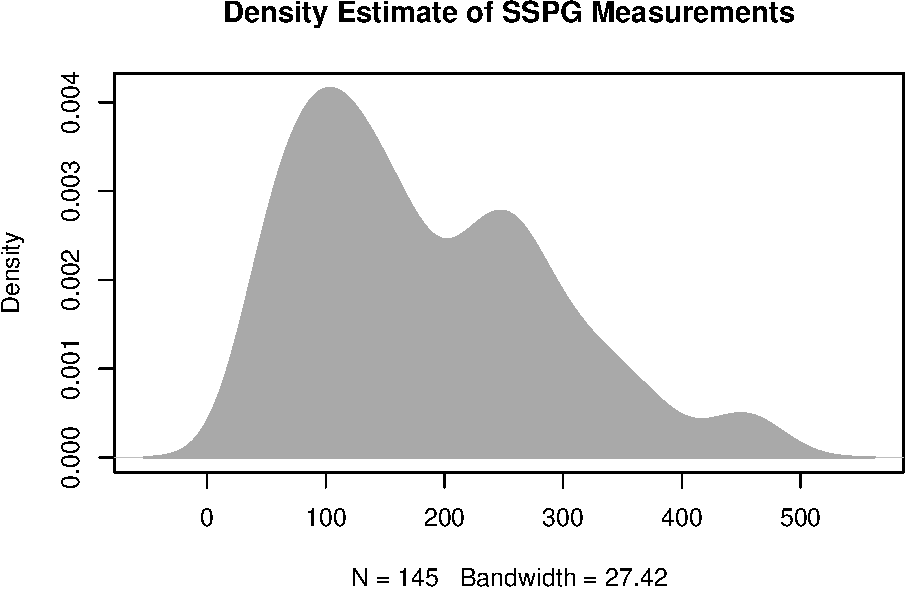
\includegraphics{a4_solutions_files/figure-latex/unnamed-chunk-2-1.pdf}

The density is right-skewed and trimodal, with modes at about 100, 250
and 450. The curve rises quickly to the first mode, then gradually
decreases. In addition, the majority of patients have an SSG measurement
below 250. Lastly, the SSPG seems lacks normality - i.e.~it does not
seem to have been sampled from the normal - as its density does not
resemble the symmetric bell curve of a normal density.

\item 

Construct a quantile plot of \texttt{SSPG} and comment on the shape of
its distribution.

\begin{Shaded}
\begin{Highlighting}[]
\NormalTok{sspg_vals =}\StringTok{ }\KeywordTok{sort}\NormalTok{(diabetes}\OperatorTok{$}\NormalTok{SSPG)}
\NormalTok{n =}\StringTok{ }\KeywordTok{length}\NormalTok{(sspg_vals)}
\NormalTok{p =}\StringTok{ }\KeywordTok{ppoints}\NormalTok{(n) }\CommentTok{# the proportions}

\KeywordTok{plot}\NormalTok{(}\DataTypeTok{x =}\NormalTok{ p, }\DataTypeTok{y =}\NormalTok{ sspg_vals, }\DataTypeTok{type=}\StringTok{"o"}\NormalTok{, }\DataTypeTok{lwd=}\DecValTok{2}\NormalTok{, }\DataTypeTok{col=}\StringTok{"grey10"}\NormalTok{,}
    \DataTypeTok{xlab=}\StringTok{"cumulative proportion"}\NormalTok{, }\DataTypeTok{xlim=}\KeywordTok{c}\NormalTok{(}\DecValTok{0}\NormalTok{,}\DecValTok{1}\NormalTok{),}
    \DataTypeTok{ylab=}\StringTok{"SSPG"}\NormalTok{, }\DataTypeTok{main=}\StringTok{"Quantile Plot of SSPG Measurements"}\NormalTok{)}
\end{Highlighting}
\end{Shaded}

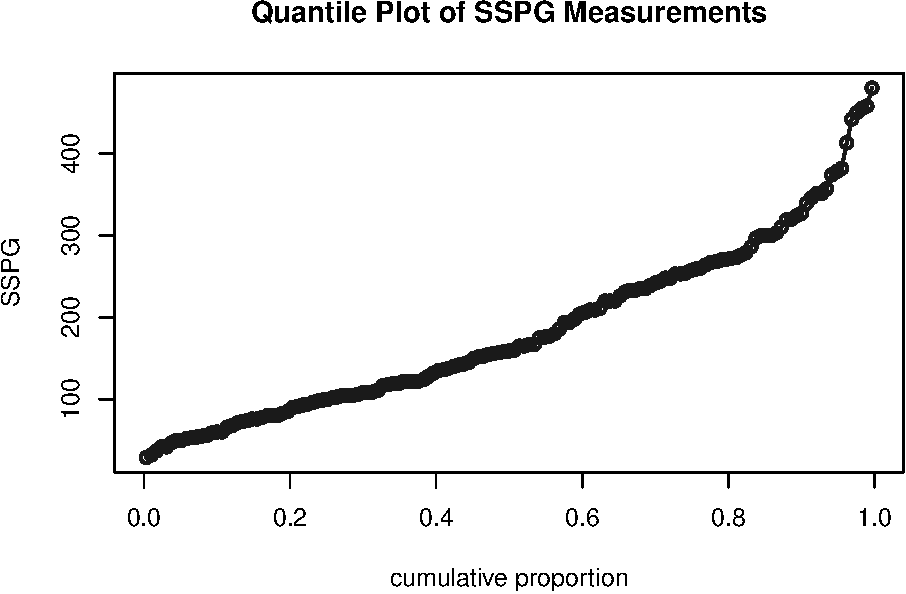
\includegraphics{a4_solutions_files/figure-latex/unnamed-chunk-3-1.pdf}

The shape of the quantile plot is nearly linear up until about the 60th
percentile, at which point it begins to curve upwards. The data seems to
be evenly concentraed throughout the plot, with sparsity at the right
tail. This indicates a lot of variation between the extremes as the
concentration of points at the left tail of the plot is relatively
higher. Overall, the plot has a convex, trough-down shape.

\item 

(3 marks) Use \texttt{qqtest} to construct a qqplot that compares
\texttt{SSPG} to a standard normal distribution. Include envelopes in
the plot. Comment on the distribution of \texttt{SSPG} and whether it
might reasonably be regarded as a sample from some normal distribution.
Explain your reasoning.

\textbf{Important:} Before every \texttt{qqtest} execute
\texttt{set.seed(3124159)} so that we are all seeing the same plots.

\begin{Shaded}
\begin{Highlighting}[]
\KeywordTok{library}\NormalTok{(qqtest)}
\CommentTok{# Setting the seed}
\KeywordTok{set.seed}\NormalTok{(}\DecValTok{3124159}\NormalTok{)}
\KeywordTok{qqtest}\NormalTok{(}\DataTypeTok{data=}\NormalTok{diabetes}\OperatorTok{$}\NormalTok{SSPG)}
\end{Highlighting}
\end{Shaded}

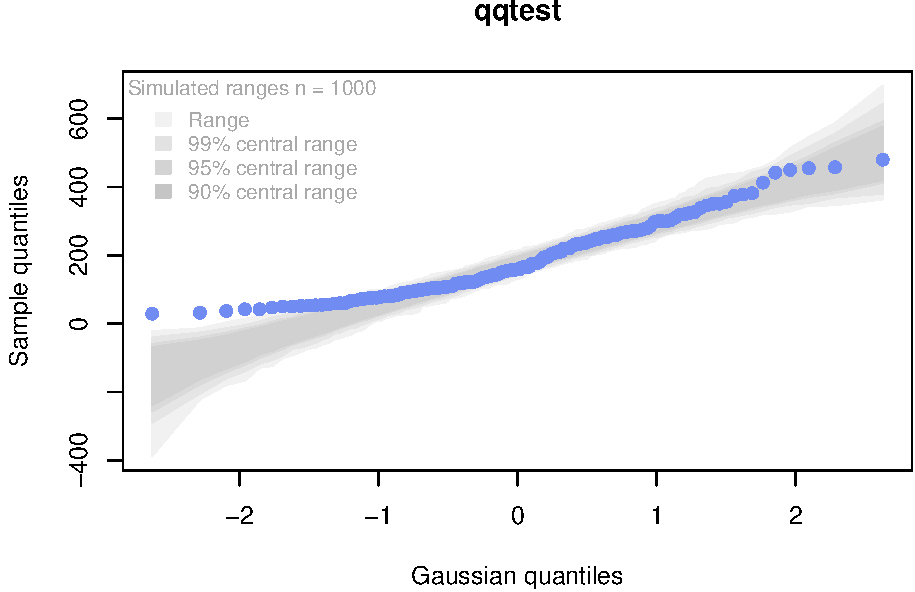
\includegraphics{a4_solutions_files/figure-latex/unnamed-chunk-4-1.pdf}

As can be seen in the plot, all the points fall within the envelope,
with the exception of the points at the left tail. However, it's on
average expected that \(n/10 = 14.5 \approx 15\) points would fall
outside of the envelope even if the SSPG was from a normal distribution,
and the points outside the envelope still lie very close to it. Hence,
using the \texttt{qqtest} results, it would be reasonable to regard the
SSPG values as a sample from a normal distribution.

\item 

The last variate, \texttt{ClinClass}, represents the classification of
each patient according to the 1979 medical criteria into one of three
groups: 1 = ``Overt Diabetic'', 2 = ``Chemical Diabetic'', and 3 =
``Normal''.

\benum     \item (4 marks) Construct a back to back density line-up plot
to assess whether the normal and diabetic (chemical and overt combined)
\texttt{SSPG} values come from the same distribution. Use
\texttt{set.seed(3124159)} and show your code. What conclusions do you
draw?

\begin{Shaded}
\begin{Highlighting}[]
\NormalTok{normal_SSPG =}\StringTok{ }\NormalTok{diabetes[diabetes}\OperatorTok{$}\NormalTok{ClinClass }\OperatorTok{==}\StringTok{ }\DecValTok{3}\NormalTok{,]}\OperatorTok{$}\NormalTok{SSPG}
\NormalTok{diabetic_SSPG =}\StringTok{ }\NormalTok{diabetes[diabetes}\OperatorTok{$}\NormalTok{ClinClass }\OperatorTok{!=}\StringTok{ }\DecValTok{3}\NormalTok{,]}\OperatorTok{$}\NormalTok{SSPG}

\NormalTok{back2back <-}\StringTok{ }\ControlFlowTok{function}\NormalTok{(data, suspectNo) \{}
\NormalTok{  ylim =}\StringTok{ }\KeywordTok{extendrange}\NormalTok{(}\KeywordTok{c}\NormalTok{(data}\OperatorTok{$}\NormalTok{x, data}\OperatorTok{$}\NormalTok{y)) }\CommentTok{#c(0,600)}
\NormalTok{  Xdensity =}\StringTok{ }\KeywordTok{density}\NormalTok{(data}\OperatorTok{$}\NormalTok{x, }\DataTypeTok{bw=}\StringTok{"SJ"}\NormalTok{)}
\NormalTok{  Ydensity =}\StringTok{ }\KeywordTok{density}\NormalTok{(data}\OperatorTok{$}\NormalTok{y, }\DataTypeTok{bw=}\StringTok{"SJ"}\NormalTok{)}
\NormalTok{  Ydensity}\OperatorTok{$}\NormalTok{y =}\StringTok{ }\OperatorTok{-}\NormalTok{Ydensity}\OperatorTok{$}\NormalTok{y}
\NormalTok{  xlim =}\StringTok{ }\KeywordTok{extendrange}\NormalTok{(}\KeywordTok{c}\NormalTok{(Xdensity}\OperatorTok{$}\NormalTok{y, Ydensity}\OperatorTok{$}\NormalTok{y))}
  
\NormalTok{  xyswitch <-}\StringTok{ }\ControlFlowTok{function}\NormalTok{(xy_plot) \{}
\NormalTok{    yx_plot =}\StringTok{ }\NormalTok{xy_plot}
\NormalTok{    yx_plot}\OperatorTok{$}\NormalTok{x =}\StringTok{ }\NormalTok{xy_plot}\OperatorTok{$}\NormalTok{y}
\NormalTok{    yx_plot}\OperatorTok{$}\NormalTok{y =}\StringTok{ }\NormalTok{xy_plot}\OperatorTok{$}\NormalTok{x}
\NormalTok{    yx_plot}
\NormalTok{  \}}
  
  \KeywordTok{plot}\NormalTok{(}\KeywordTok{xyswitch}\NormalTok{(Xdensity), }\DataTypeTok{col=}\StringTok{"firebrick"}\NormalTok{,}
       \DataTypeTok{xlab=}\StringTok{""}\NormalTok{, }\DataTypeTok{ylab=}\StringTok{""}\NormalTok{, }\DataTypeTok{xaxt=}\StringTok{"n"}\NormalTok{, }\DataTypeTok{yaxt=}\StringTok{"n"}\NormalTok{,}
       \DataTypeTok{main=}\KeywordTok{paste}\NormalTok{(}\StringTok{"i = "}\NormalTok{, suspectNo),}\CommentTok{# display suspect number}
       \DataTypeTok{cex.main =} \DecValTok{2}\NormalTok{, }\CommentTok{# increase suspect number size}
       \DataTypeTok{xlim=}\NormalTok{xlim, }\DataTypeTok{ylim=}\NormalTok{ylim)}
  \KeywordTok{polygon}\NormalTok{(}\KeywordTok{xyswitch}\NormalTok{(Xdensity), }\DataTypeTok{col=}\KeywordTok{adjustcolor}\NormalTok{(}\StringTok{"firebrick"}\NormalTok{, }\FloatTok{0.4}\NormalTok{))}
  \KeywordTok{lines}\NormalTok{(}\KeywordTok{xyswitch}\NormalTok{(Ydensity), }\DataTypeTok{col=}\StringTok{"steelblue"}\NormalTok{)}
  \KeywordTok{polygon}\NormalTok{(}\KeywordTok{xyswitch}\NormalTok{(Ydensity), }\DataTypeTok{col=}\KeywordTok{adjustcolor}\NormalTok{(}\StringTok{"steelblue"}\NormalTok{,}\FloatTok{0.4}\NormalTok{))}
\NormalTok{\}}

\NormalTok{mixRandomly <-}\StringTok{ }\ControlFlowTok{function}\NormalTok{(data) \{}
  \CommentTok{# Note that data need not be a data frame}
  \CommentTok{# It is expected to be a list with an x and a y component}
  \CommentTok{# (possibly of different lengths)}
\NormalTok{  x <-}\StringTok{ }\NormalTok{data}\OperatorTok{$}\NormalTok{x}
\NormalTok{  y <-}\StringTok{ }\NormalTok{data}\OperatorTok{$}\NormalTok{y}
\NormalTok{  n_x <-}\KeywordTok{length}\NormalTok{(x)}
\NormalTok{  n_y <-}\KeywordTok{length}\NormalTok{(y)}
\NormalTok{  mix <-}\KeywordTok{c}\NormalTok{(x,y)}
\NormalTok{  select4x <-}\KeywordTok{sample}\NormalTok{(}\DecValTok{1}\OperatorTok{:}\NormalTok{(n_x}\OperatorTok{+}\NormalTok{n_y),n_x,}\DataTypeTok{replace =} \OtherTok{FALSE}\NormalTok{)}
\NormalTok{  new_x <-}\StringTok{ }\NormalTok{mix[select4x] }\CommentTok{# The mixing occurs}
\NormalTok{  new_y <-}\StringTok{ }\NormalTok{mix[}\OperatorTok{-}\NormalTok{select4x]}
  \KeywordTok{list}\NormalTok{(}\DataTypeTok{x=}\NormalTok{new_x, }\DataTypeTok{y=}\NormalTok{new_y)}
\NormalTok{\}}

\NormalTok{lineup <-}\StringTok{ }\ControlFlowTok{function}\NormalTok{(data, }\DataTypeTok{showSuspect=}\OtherTok{NULL}\NormalTok{, }\DataTypeTok{generateSuspect=}\OtherTok{NULL}\NormalTok{,}
                   \DataTypeTok{trueLoc=}\OtherTok{NULL}\NormalTok{, }\DataTypeTok{layout =}\KeywordTok{c}\NormalTok{(}\DecValTok{5}\NormalTok{,}\DecValTok{4}\NormalTok{)) \{}
  \CommentTok{# Get the number of suspects in total}
\NormalTok{  nSuspects <-}\StringTok{ }\NormalTok{layout[}\DecValTok{1}\NormalTok{] }\OperatorTok{*}\StringTok{ }\NormalTok{layout[}\DecValTok{2}\NormalTok{]}
  \ControlFlowTok{if}\NormalTok{ (}\KeywordTok{is.null}\NormalTok{(trueLoc)) \{trueLoc <-}\KeywordTok{sample}\NormalTok{(}\DecValTok{1}\OperatorTok{:}\NormalTok{nSuspects, }\DecValTok{1}\NormalTok{)\}}
  \ControlFlowTok{if}\NormalTok{ (}\KeywordTok{is.null}\NormalTok{(showSuspect)) \{}\KeywordTok{stop}\NormalTok{(}\StringTok{"need a plot function for the suspect"}\NormalTok{)\}}
  \ControlFlowTok{if}\NormalTok{ (}\KeywordTok{is.null}\NormalTok{(generateSuspect)) \{}\KeywordTok{stop}\NormalTok{(}\StringTok{"need a function to generate suspect"}\NormalTok{)\}}
  \CommentTok{# Need to decide which subject to present}
\NormalTok{  presentSuspect <-}\StringTok{ }\ControlFlowTok{function}\NormalTok{(suspectNo) \{}
    \ControlFlowTok{if}\NormalTok{(suspectNo }\OperatorTok{!=}\StringTok{ }\NormalTok{trueLoc) \{data <-}\KeywordTok{generateSuspect}\NormalTok{(data)\}}
    \KeywordTok{showSuspect}\NormalTok{(data, suspectNo) }
\NormalTok{  \}}
  \CommentTok{# This does the plotting}
\NormalTok{  savePar <-}\KeywordTok{par}\NormalTok{(}\DataTypeTok{mfrow=}\NormalTok{layout,}\DataTypeTok{mar=}\KeywordTok{c}\NormalTok{(}\FloatTok{2.5}\NormalTok{, }\FloatTok{0.1}\NormalTok{, }\DecValTok{3}\NormalTok{, }\FloatTok{0.1}\NormalTok{), }\DataTypeTok{oma=}\KeywordTok{rep}\NormalTok{(}\DecValTok{0}\NormalTok{,}\DecValTok{4}\NormalTok{))}
  \KeywordTok{sapply}\NormalTok{(}\DecValTok{1}\OperatorTok{:}\NormalTok{nSuspects, }\DataTypeTok{FUN =}\NormalTok{ presentSuspect)}
  \KeywordTok{par}\NormalTok{(savePar)}
  
  \CommentTok{# Obfuscate location to keep us honest}
\NormalTok{  possibleBaseVals <-}\StringTok{ }\DecValTok{3}\OperatorTok{:}\KeywordTok{min}\NormalTok{(}\DecValTok{2}\OperatorTok{*}\NormalTok{nSuspects, }\DecValTok{50}\NormalTok{) }\CommentTok{# remove easy base values}
\NormalTok{  possibleBaseVals <-}\StringTok{ }\NormalTok{possibleBaseVals[possibleBaseVals }\OperatorTok{!=}\StringTok{ }\DecValTok{10} \OperatorTok{&}\StringTok{ }\NormalTok{possibleBaseVals }\OperatorTok{!=}\StringTok{ }\DecValTok{5}\NormalTok{]}
\NormalTok{  base <-}\KeywordTok{sample}\NormalTok{(possibleBaseVals, }\DecValTok{1}\NormalTok{)}
\NormalTok{  offset <-}\KeywordTok{sample}\NormalTok{(}\DecValTok{5}\OperatorTok{:}\KeywordTok{min}\NormalTok{(}\DecValTok{5}\OperatorTok{*}\NormalTok{nSuspects, }\DecValTok{125}\NormalTok{),}\DecValTok{1}\NormalTok{)}
  
  \CommentTok{# return obfuscated location}
  \KeywordTok{list}\NormalTok{(}\DataTypeTok{trueLoc =}\KeywordTok{paste0}\NormalTok{(}\StringTok{"log("}\NormalTok{,base}\OperatorTok{^}\NormalTok{(trueLoc }\OperatorTok{+}\StringTok{ }\NormalTok{offset),}
                       \StringTok{", base="}\NormalTok{,base,}\StringTok{") - "}\NormalTok{, offset))}
\NormalTok{\}}

\NormalTok{data =}\StringTok{ }\KeywordTok{list}\NormalTok{(}\DataTypeTok{x=}\NormalTok{normal_SSPG, }\DataTypeTok{y=}\NormalTok{diabetic_SSPG)}
\KeywordTok{set.seed}\NormalTok{(}\DecValTok{3124159}\NormalTok{)}
\KeywordTok{lineup}\NormalTok{(data,}
       \DataTypeTok{generateSuspect =}\NormalTok{ mixRandomly,}
       \DataTypeTok{showSuspect =}\NormalTok{ back2back)}
\end{Highlighting}
\end{Shaded}

\begin{center}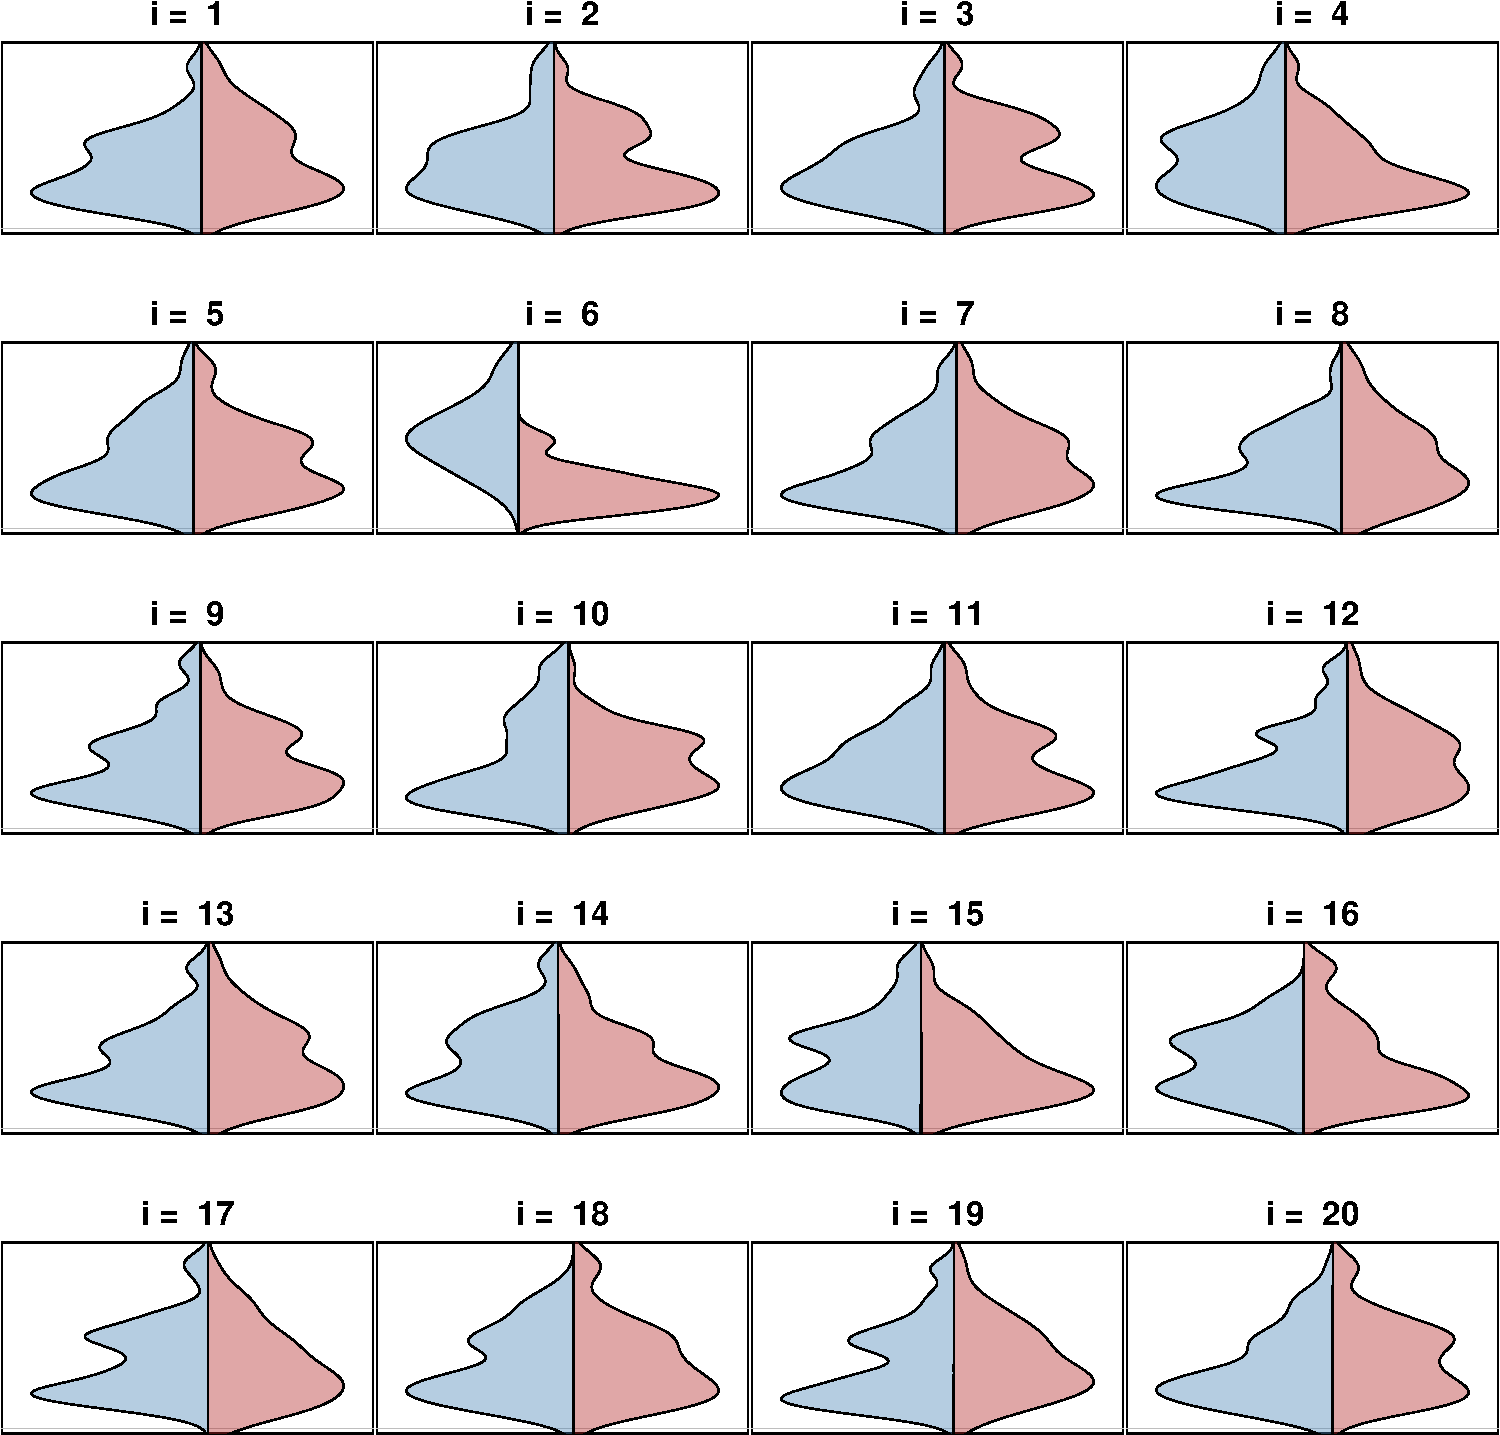
\includegraphics{a4_solutions_files/figure-latex/unnamed-chunk-5-1} \end{center}

\begin{verbatim}
## $trueLoc
## [1] "log(7.51141330201283e+30, base=22) - 17"
\end{verbatim}

From the lineup test, it is visually clear that the true plot is at
\(i = 6\) - which is indeed equal to the generated value of
\texttt{trueLoc} - as this plot stands out more than any of the others.
Hence, using this lineup test, there is enough evidence to reject the
hypothesis that the two sets come from the same-shaped distribution.

\item 

(4 marks) Use \texttt{qqtest} to construct a lineup plot making the same
assessment, but this time assess whether the overt diabetic values of
\texttt{SSPG} might have been generated from the same distribution as
the normal patients. Use \texttt{set.seed(3124159)} and show your code.
What conclusions do you draw?

\begin{Shaded}
\begin{Highlighting}[]
\KeywordTok{set.seed}\NormalTok{(}\DecValTok{3124159}\NormalTok{)}
\NormalTok{overt_SSPG =}\StringTok{ }\NormalTok{diabetes[diabetes}\OperatorTok{$}\NormalTok{ClinClass }\OperatorTok{==}\StringTok{ }\DecValTok{1}\NormalTok{,]}\OperatorTok{$}\NormalTok{SSPG}
\KeywordTok{qqtest}\NormalTok{(}\DataTypeTok{data =}\NormalTok{ overt_SSPG, }\DataTypeTok{dataTest=}\NormalTok{normal_SSPG,}
       \DataTypeTok{lineup=}\OtherTok{TRUE}\NormalTok{)}
\end{Highlighting}
\end{Shaded}

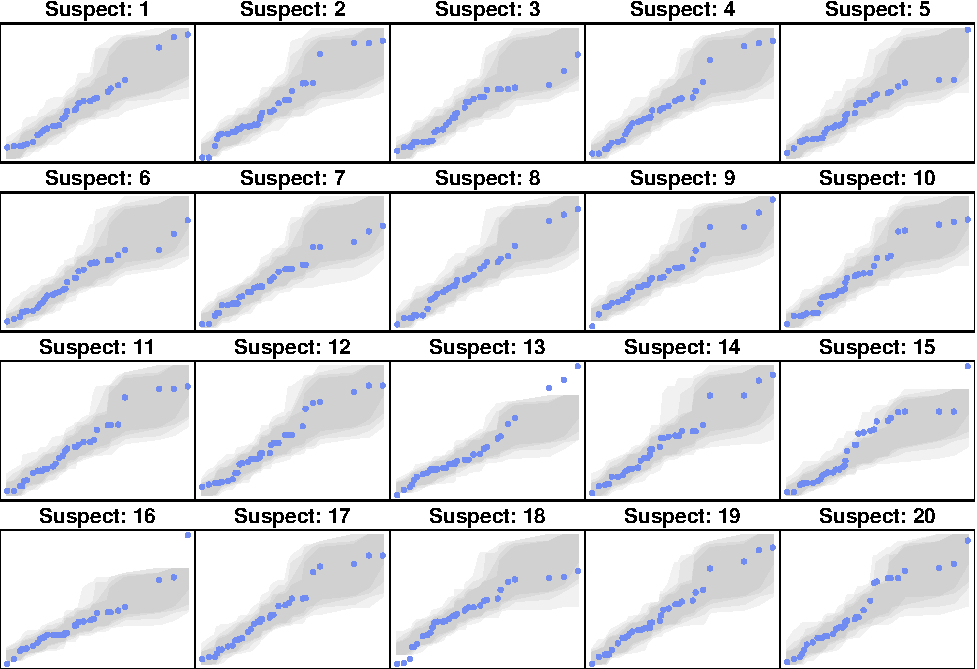
\includegraphics{a4_solutions_files/figure-latex/unnamed-chunk-6-1.pdf}

\begin{verbatim}
## $TrueLoc
## [1] "log(2.90474294739124e+100, base=26) - 53"
\end{verbatim}

It is difficult to see a significant difference between any of the
plots. Plot 16 stands out the most personally, but this differs from the
\texttt{trueLoc} at \(18\). Hence, using this lineup test, even though
in all plots the overt diabetic SSPG values fall within the envelope,
there is not enough evidence to reject the hypothesis that the overt
diabetic values of \texttt{SSPG} might have been generated from the same
distribution as the normal patients. The qqtests seem to be producing a
type II error.

\item 

\textbf{Grad students, bonus undergraduates} (8 marks) Consider the
following code:

\begin{Shaded}
\begin{Highlighting}[]
\NormalTok{data <-}\StringTok{ }\KeywordTok{list}\NormalTok{(}\DataTypeTok{x=}\NormalTok{x, }\DataTypeTok{y=}\NormalTok{y, }\DataTypeTok{z=}\NormalTok{z)}
\KeywordTok{lineup}\NormalTok{(data, }
\DataTypeTok{generateSuspect =}\NormalTok{ mixRandomly, }
\DataTypeTok{showSuspect =}\NormalTok{ myQuantilePlot, }
\DataTypeTok{layout=}\KeywordTok{c}\NormalTok{(}\DecValTok{5}\NormalTok{,}\DecValTok{4}\NormalTok{))}
\end{Highlighting}
\end{Shaded}

The function \texttt{mixRandomly} will need to be rewritten to handle
\texttt{data} being a list of three samples. Write the function
\texttt{myQuantilePlot} so that it overlays the sample quantile
functions of each of \texttt{x}, \texttt{y}, and \texttt{z} in the same
display using different colours. Hand in your code for these two
functions and illustrate the outcome (using \texttt{set.seed(314159)})
on \texttt{SSPG} for the three different clinical classes. Comment on
your findings.

\begin{Shaded}
\begin{Highlighting}[]
\NormalTok{mixRandomly <-}\StringTok{ }\ControlFlowTok{function}\NormalTok{(data) \{}
  \CommentTok{# Note that data need not be a data frame}
  \CommentTok{# It is expected to be a list with an x, a y and a z component}
  \CommentTok{# (possibly of different lengths)}
\NormalTok{  x =}\StringTok{ }\NormalTok{data}\OperatorTok{$}\NormalTok{x}
\NormalTok{  y =}\StringTok{ }\NormalTok{data}\OperatorTok{$}\NormalTok{y}
\NormalTok{  z =}\StringTok{ }\NormalTok{data}\OperatorTok{$}\NormalTok{z}
\NormalTok{  n_x =}\StringTok{ }\KeywordTok{length}\NormalTok{(x)}
\NormalTok{  n_y =}\StringTok{ }\KeywordTok{length}\NormalTok{(y)}
\NormalTok{  n_z =}\StringTok{ }\KeywordTok{length}\NormalTok{(y)}
\NormalTok{  mix =}\StringTok{ }\KeywordTok{c}\NormalTok{(x,y,z)}
\NormalTok{  full_range =}\StringTok{ }\DecValTok{1}\OperatorTok{:}\NormalTok{(n_x}\OperatorTok{+}\NormalTok{n_y}\OperatorTok{+}\NormalTok{n_z)}
\NormalTok{  select4x =}\StringTok{ }\KeywordTok{sample}\NormalTok{(full_range,n_x,}\DataTypeTok{replace =} \OtherTok{FALSE}\NormalTok{)}
  \CommentTok{# remove indices in select4x from sampling pool and sample indices for y}
\NormalTok{  select4y =}\StringTok{ }\KeywordTok{sample}\NormalTok{(full_range[}\OperatorTok{-}\NormalTok{select4x],n_y,}\DataTypeTok{replace =} \OtherTok{FALSE}\NormalTok{)}
\NormalTok{  new_x =}\StringTok{ }\NormalTok{mix[select4x] }\CommentTok{# The mixing occurs}
\NormalTok{  new_y =}\StringTok{ }\NormalTok{mix[select4y]}
\NormalTok{  new_z =}\StringTok{ }\NormalTok{mix[}\OperatorTok{-}\NormalTok{select4y] }
  \KeywordTok{list}\NormalTok{(}\DataTypeTok{x=}\NormalTok{new_x, }\DataTypeTok{y=}\NormalTok{new_y, }\DataTypeTok{z=}\NormalTok{new_z)}
\NormalTok{\}}

\CommentTok{# should there be an option to specify colors or can we choose any?}
\NormalTok{myQuantilePlot <-}\StringTok{ }\ControlFlowTok{function}\NormalTok{(data, suspectNo) \{}
\NormalTok{  ylim =}\StringTok{ }\KeywordTok{extendrange}\NormalTok{(}\KeywordTok{c}\NormalTok{(data}\OperatorTok{$}\NormalTok{x, data}\OperatorTok{$}\NormalTok{y, data}\OperatorTok{$}\NormalTok{z))}
\NormalTok{  n_x =}\StringTok{ }\KeywordTok{length}\NormalTok{(data}\OperatorTok{$}\NormalTok{x)}
\NormalTok{  n_y =}\StringTok{ }\KeywordTok{length}\NormalTok{(data}\OperatorTok{$}\NormalTok{y)}
\NormalTok{  n_z =}\StringTok{ }\KeywordTok{length}\NormalTok{(data}\OperatorTok{$}\NormalTok{z)}
\NormalTok{  p_x =}\StringTok{ }\KeywordTok{ppoints}\NormalTok{(n_x)}
\NormalTok{  p_y =}\StringTok{ }\KeywordTok{ppoints}\NormalTok{(n_y)}
\NormalTok{  p_z =}\StringTok{ }\KeywordTok{ppoints}\NormalTok{(n_z)}
  \KeywordTok{plot}\NormalTok{(p_x, }\KeywordTok{sort}\NormalTok{(data}\OperatorTok{$}\NormalTok{x), }\DataTypeTok{type=}\StringTok{"b"}\NormalTok{, }\DataTypeTok{col=}\KeywordTok{adjustcolor}\NormalTok{(}\StringTok{"firebrick"}\NormalTok{, }\FloatTok{0.4}\NormalTok{),  }
       \DataTypeTok{pch=}\DecValTok{19}\NormalTok{, }\DataTypeTok{cex=}\DecValTok{2}\NormalTok{, }\DataTypeTok{ylim =}\NormalTok{ ylim,}
       \DataTypeTok{main=}\KeywordTok{paste}\NormalTok{(}\StringTok{"i ="}\NormalTok{, suspectNo), }\CommentTok{# display suspect number}
       \DataTypeTok{cex.main =} \DecValTok{3}\NormalTok{,}\CommentTok{# increase suspect number size}
       \DataTypeTok{ylab=}\StringTok{""}\NormalTok{, }\DataTypeTok{xlab=}\StringTok{""}\NormalTok{, }\DataTypeTok{xaxt=}\StringTok{"n"}\NormalTok{, }\DataTypeTok{yaxt=}\StringTok{"n"}\NormalTok{)}
  \KeywordTok{points}\NormalTok{(p_y,}\KeywordTok{sort}\NormalTok{(data}\OperatorTok{$}\NormalTok{y), }\DataTypeTok{type=}\StringTok{"b"}\NormalTok{,}
         \DataTypeTok{col=}\KeywordTok{adjustcolor}\NormalTok{(}\StringTok{"steelblue"}\NormalTok{, }\FloatTok{0.4}\NormalTok{),  }\DataTypeTok{pch=}\DecValTok{19}\NormalTok{, }\DataTypeTok{cex=}\DecValTok{2}\NormalTok{)}
  \KeywordTok{points}\NormalTok{(p_z,}\KeywordTok{sort}\NormalTok{(data}\OperatorTok{$}\NormalTok{z), }\DataTypeTok{type=}\StringTok{"b"}\NormalTok{,}
         \DataTypeTok{col=}\KeywordTok{adjustcolor}\NormalTok{(}\StringTok{"yellowgreen"}\NormalTok{, }\FloatTok{0.4}\NormalTok{),  }\DataTypeTok{pch=}\DecValTok{19}\NormalTok{, }\DataTypeTok{cex=}\DecValTok{2}\NormalTok{)}
\NormalTok{\}}

\NormalTok{chemical_SSPG =}\StringTok{ }\NormalTok{diabetes[diabetes}\OperatorTok{$}\NormalTok{ClinClass }\OperatorTok{==}\StringTok{ }\DecValTok{2}\NormalTok{,]}\OperatorTok{$}\NormalTok{SSPG}
\NormalTok{sspg_data =}\StringTok{ }\KeywordTok{list}\NormalTok{(}\DataTypeTok{x=}\NormalTok{overt_SSPG, }\DataTypeTok{y=}\NormalTok{chemical_SSPG, }\DataTypeTok{z=}\NormalTok{normal_SSPG)}
\KeywordTok{set.seed}\NormalTok{(}\DecValTok{314159}\NormalTok{)}
\KeywordTok{lineup}\NormalTok{(sspg_data, }
        \DataTypeTok{generateSuspect =}\NormalTok{ mixRandomly, }
        \DataTypeTok{showSuspect =}\NormalTok{ myQuantilePlot, }
        \DataTypeTok{layout=}\KeywordTok{c}\NormalTok{(}\DecValTok{5}\NormalTok{,}\DecValTok{4}\NormalTok{))}
\end{Highlighting}
\end{Shaded}

\begin{center}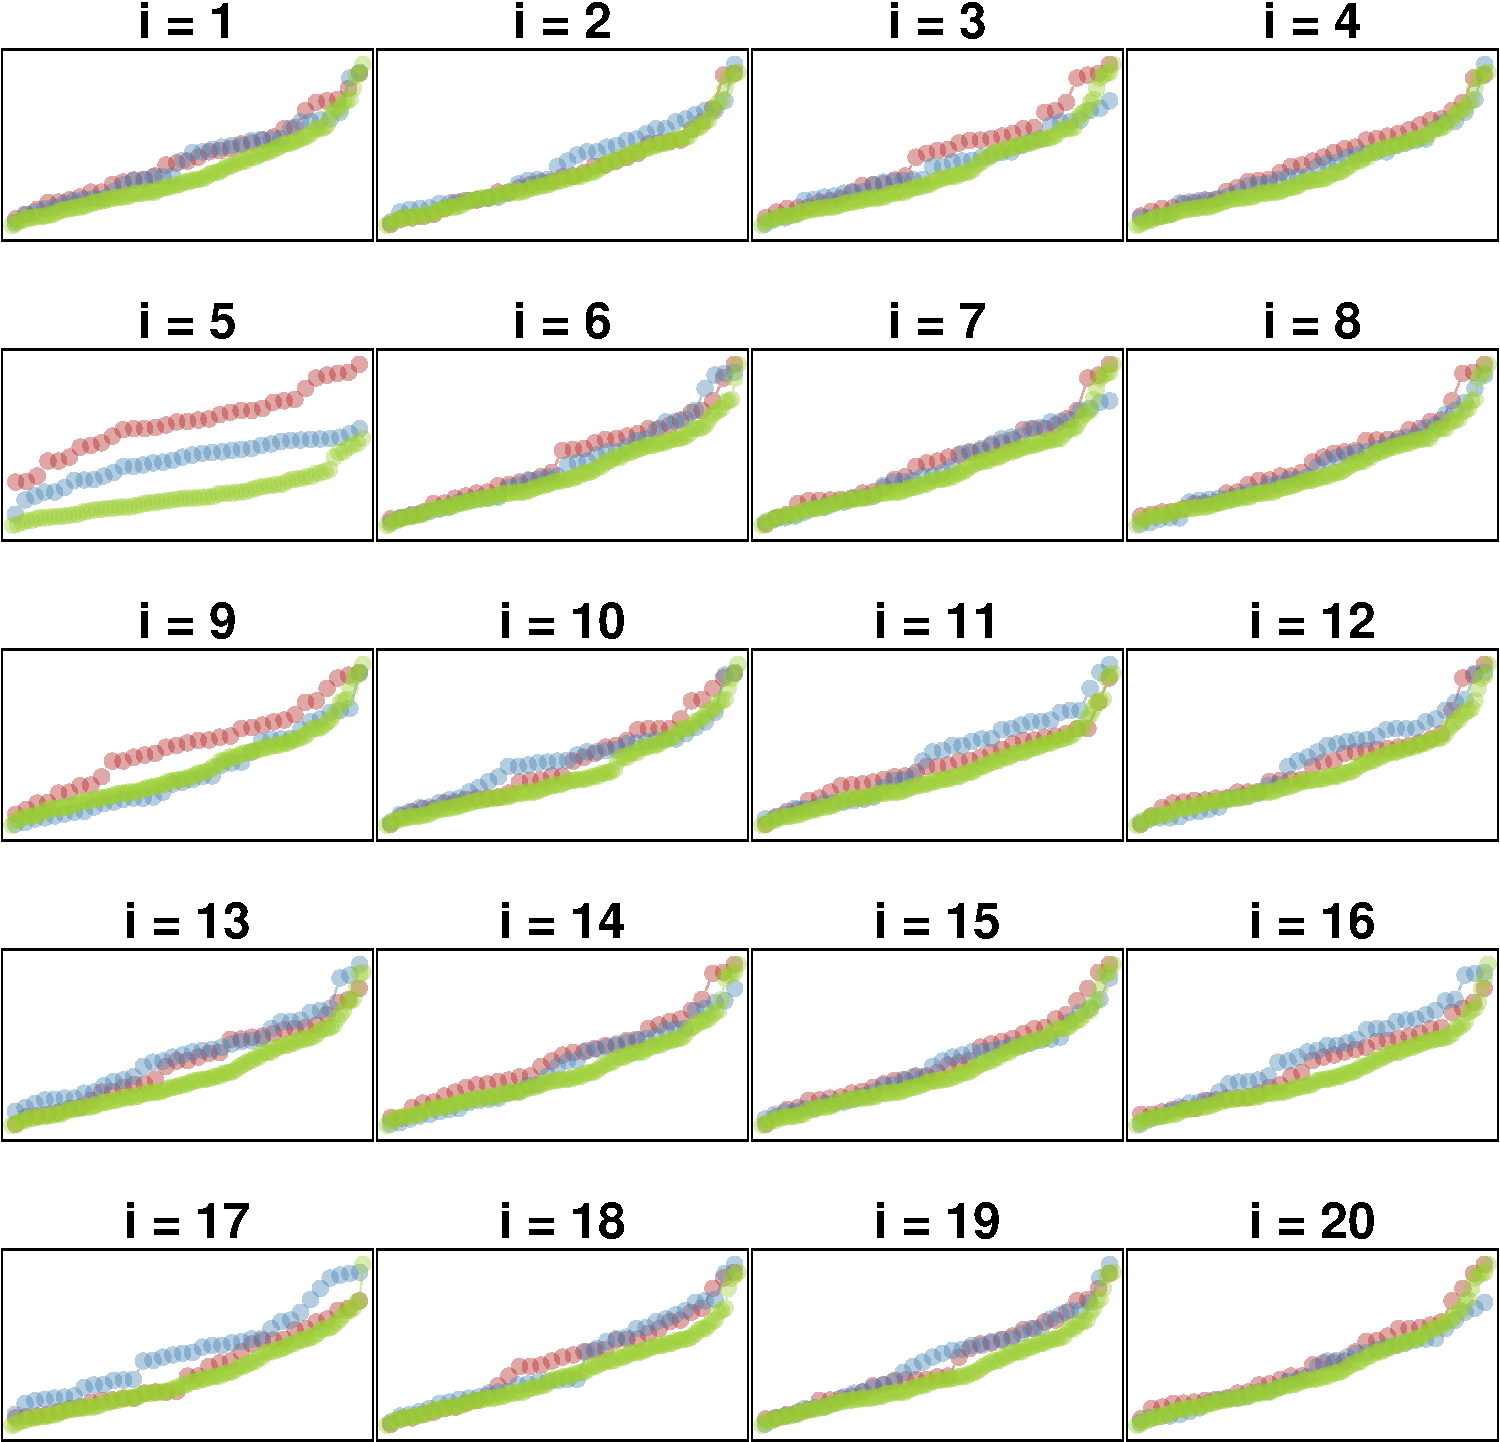
\includegraphics{a4_solutions_files/figure-latex/unnamed-chunk-8-1} \end{center}

\begin{verbatim}
## $trueLoc
## [1] "log(6.6790315523026e+66, base=39) - 37"
\end{verbatim}

From the lineup test, it is visually clear that the true plot is at
\(i = 5\) - which is indeed equal to the generated value of
\texttt{trueLoc} - as in this plot, none of the graphs never overlap
unlike every other plot. Hence, using this lineup test, there is enough
evidence to reject the hypothesis that the three sets come from the
same-shaped distribution.

\eenum
\eenum

\item 

Download the \texttt{olive} data from the course website. In that file,
there is a dataset on the fatty acid content of 572 different Italian
olive oils. In total eight different fatty acids are measured. All olive
oils come from one of nine different olive growing regions in Italy.

\begin{center}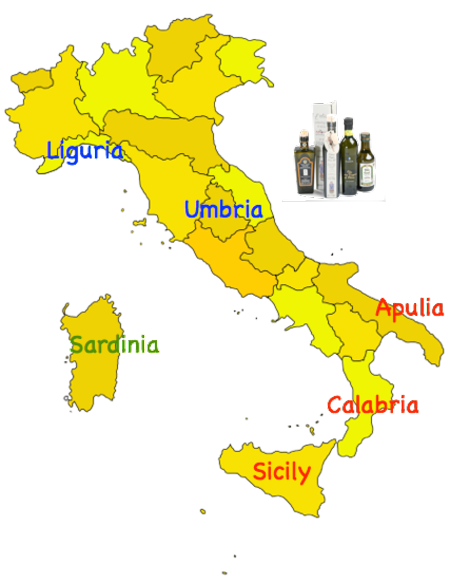
\includegraphics{a4_solutions_files/figure-latex/unnamed-chunk-9-1} \end{center}

Once you load this file into your \texttt{R} session there will be a
data set called \texttt{olive}.

In this question you are going to focus on the fatty acid
\texttt{oleic}.

\benum
\item (2 marks) Separate the data on \texttt{oleic} into 9 different
groups as defined by the olive growing \texttt{Area}, and draw side by
side boxplots of all 9 groups. Colour the boxplots uniquely using

\begin{Shaded}
\begin{Highlighting}[]
\KeywordTok{library}\NormalTok{(colorspace)}
\NormalTok{cols <-}\StringTok{ }\KeywordTok{rainbow_hcl}\NormalTok{(}\DecValTok{9}\NormalTok{) }\CommentTok{# Use these colours.}
\end{Highlighting}
\end{Shaded}

Show your code together with your output.

\begin{Shaded}
\begin{Highlighting}[]
\NormalTok{groups =}\StringTok{ }\KeywordTok{with}\NormalTok{(olive, }\KeywordTok{split}\NormalTok{(}\KeywordTok{sqrt}\NormalTok{(oleic), Area))}
\NormalTok{ord =}\StringTok{ }\KeywordTok{order}\NormalTok{(}\KeywordTok{sapply}\NormalTok{(groups, IQR))}
\KeywordTok{boxplot}\NormalTok{(groups[ord], }\DataTypeTok{col=}\NormalTok{cols[ord], }
        \DataTypeTok{main=}\StringTok{"Olive Growing Areas in Italy"}\NormalTok{)}
\end{Highlighting}
\end{Shaded}

\begin{center}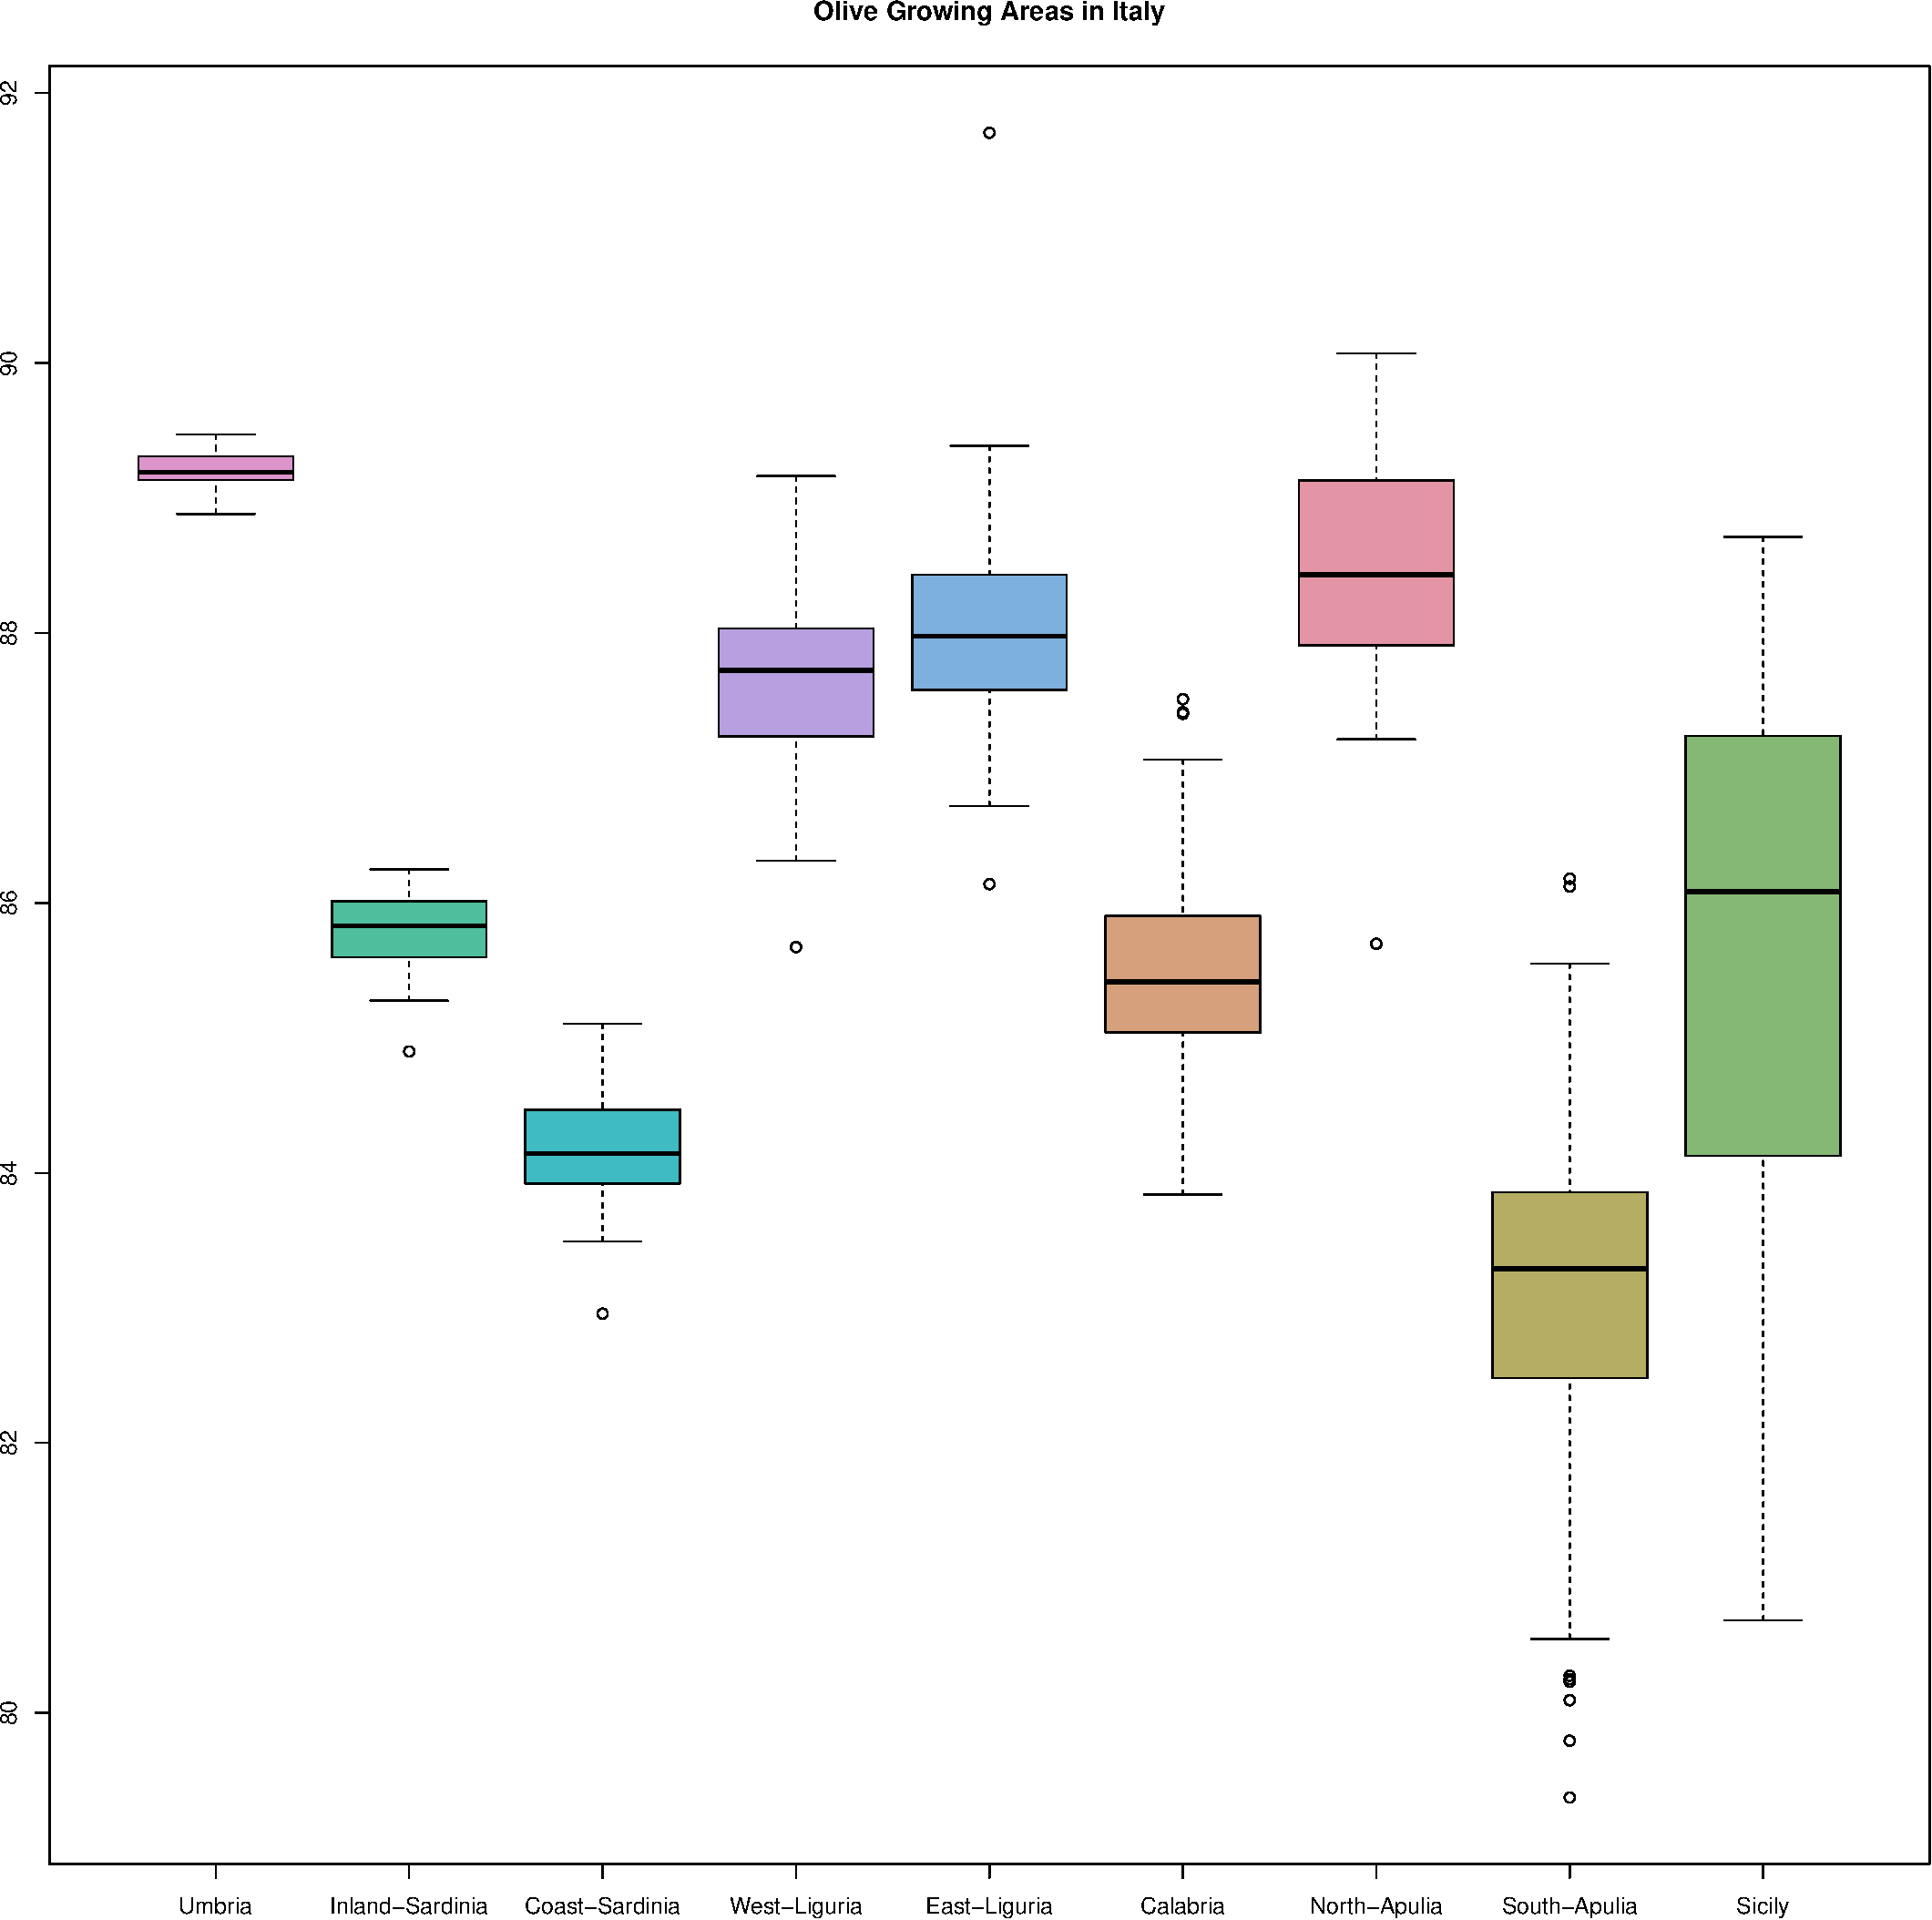
\includegraphics{a4_solutions_files/figure-latex/unnamed-chunk-12-1} \end{center}

\item 

Load the \texttt{R} package \texttt{PairViz}. Use the variate
\texttt{oleic} and the same colours for the olive growing areas as in
part (a) throughout the following:

\begin{Shaded}
\begin{Highlighting}[]
\KeywordTok{library}\NormalTok{(PairViz)}
\end{Highlighting}
\end{Shaded}

\begin{verbatim}
## Loading required package: TSP
\end{verbatim}

\begin{verbatim}
## Loading required package: gtools
\end{verbatim}

\begin{verbatim}
## Loading required package: graph
\end{verbatim}

\begin{verbatim}
## Loading required package: BiocGenerics
\end{verbatim}

\begin{verbatim}
## Loading required package: parallel
\end{verbatim}

\begin{verbatim}
## 
## Attaching package: 'BiocGenerics'
\end{verbatim}

\begin{verbatim}
## The following objects are masked from 'package:parallel':
## 
##     clusterApply, clusterApplyLB, clusterCall, clusterEvalQ,
##     clusterExport, clusterMap, parApply, parCapply, parLapply,
##     parLapplyLB, parRapply, parSapply, parSapplyLB
\end{verbatim}

\begin{verbatim}
## The following objects are masked from 'package:stats':
## 
##     IQR, mad, sd, var, xtabs
\end{verbatim}

\begin{verbatim}
## The following objects are masked from 'package:base':
## 
##     anyDuplicated, append, as.data.frame, cbind, colMeans,
##     colnames, colSums, do.call, duplicated, eval, evalq, Filter,
##     Find, get, grep, grepl, intersect, is.unsorted, lapply,
##     lengths, Map, mapply, match, mget, order, paste, pmax,
##     pmax.int, pmin, pmin.int, Position, rank, rbind, Reduce,
##     rowMeans, rownames, rowSums, sapply, setdiff, sort, table,
##     tapply, union, unique, unsplit, which, which.max, which.min
\end{verbatim}

\benum
\item (3 marks) Suppose we wish every pair of boxplots to appear next to
one another in the same plot. \bitem
\item How many such pairwise comparisons exist?

Since we do not care about the order of the boxplots in the comparisons,
the number of ways that we can choose \textbf{2} boxplots to compare out
of the total \textbf{9} is
\(C(9,2) = \frac{9!}{7!2!} = \frac{9(8)}{2} = 36\). Hence, \textbf{36}
pairwise comparisons exist.

\item 

Give the code that will construct this display (without any other
constraint on the ordering). \item Show the display which resulted from
your code.

\begin{Shaded}
\begin{Highlighting}[]
\CommentTok{# Make this bigger and shorten names}
\NormalTok{n =}\StringTok{ }\KeywordTok{length}\NormalTok{(groups)}
\NormalTok{ordEul =}\StringTok{ }\KeywordTok{eulerian}\NormalTok{(n)}
\KeywordTok{boxplot}\NormalTok{(groups[ordEul], }\DataTypeTok{col=}\NormalTok{cols[ordEul],}
        \DataTypeTok{ylab=}\KeywordTok{expression}\NormalTok{(}\KeywordTok{sqrt}\NormalTok{(}\StringTok{"Oleic Level"}\NormalTok{)),}
        \DataTypeTok{main=}\StringTok{"Oleic Levels by Olive Growing Area"}\NormalTok{)}
\end{Highlighting}
\end{Shaded}

\begin{center}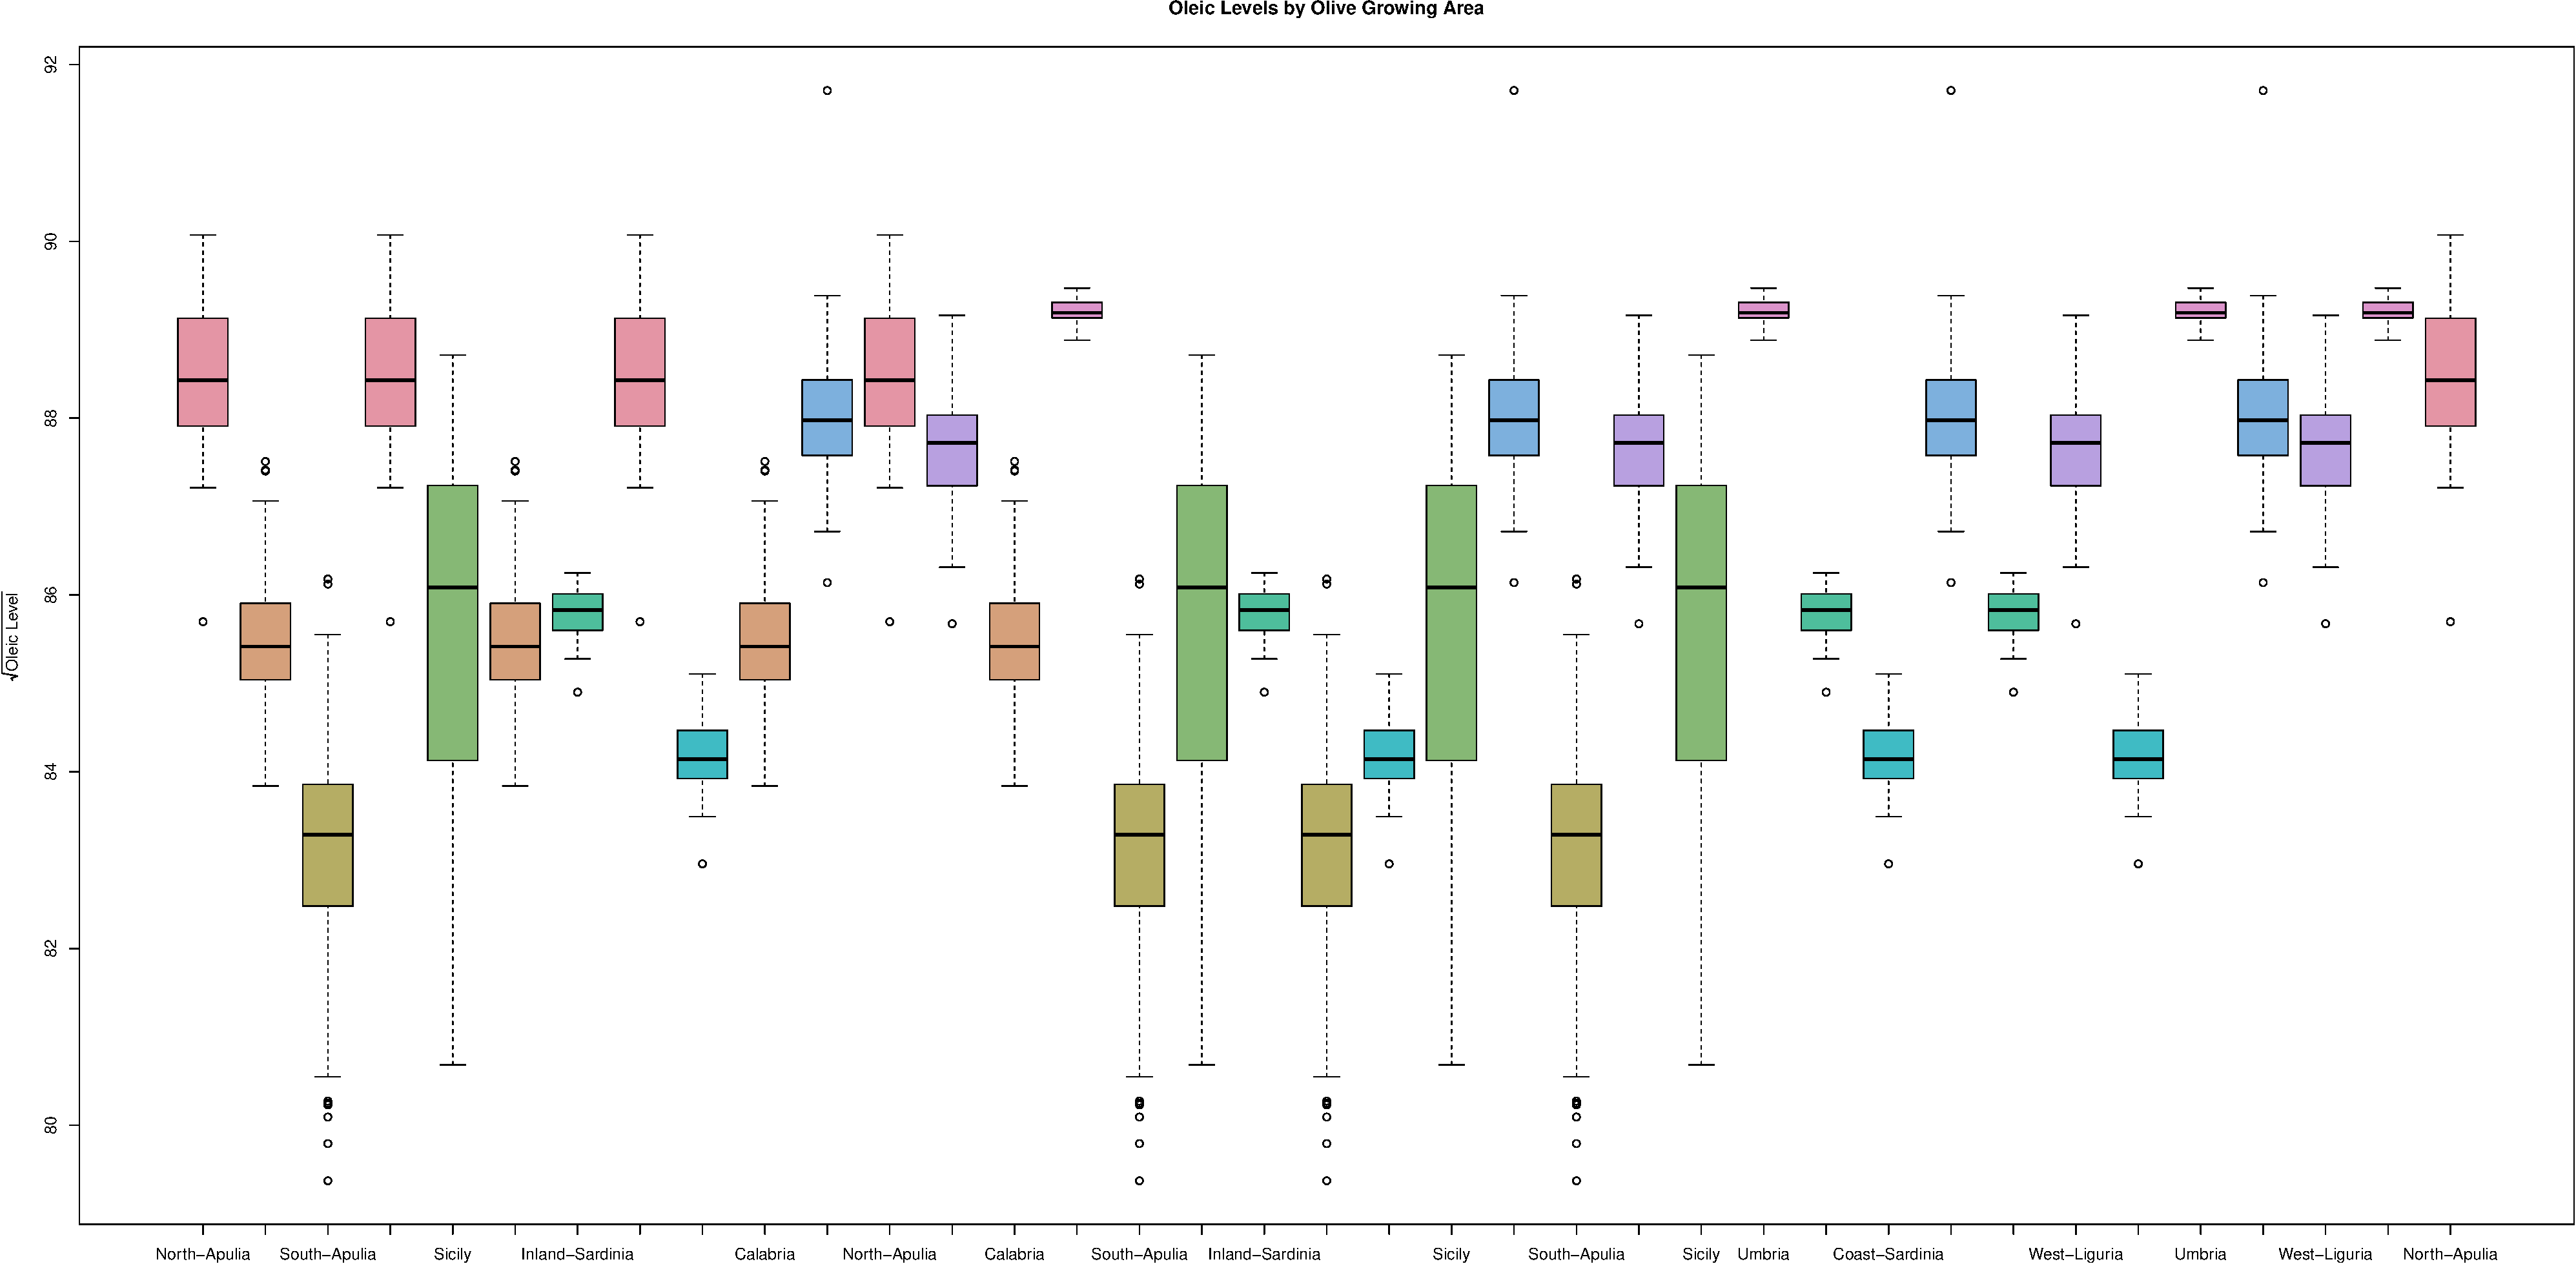
\includegraphics{a4_solutions_files/figure-latex/unnamed-chunk-14-1} \end{center}

\eitem        

\item 

(5 marks) Suppose we wish every pair of boxplots to appear next to one
another in the same plot but that the boxplots should be grouped so that
all areas appear only once in each group. \bitem
\item Maintaining the same colours for the areas as before, give the
code that will construct this display (without any other constraint on
the ordering).\\
\item Show the display which resulted from your code.

\begin{Shaded}
\begin{Highlighting}[]
\NormalTok{ordHam =}\StringTok{ }\KeywordTok{hpaths}\NormalTok{(n, }\DataTypeTok{matrix=}\OtherTok{FALSE}\NormalTok{)}
\KeywordTok{boxplot}\NormalTok{(groups[ordHam], }\DataTypeTok{col=}\NormalTok{cols[ordHam],}
        \DataTypeTok{ylab=}\KeywordTok{expression}\NormalTok{(}\KeywordTok{sqrt}\NormalTok{(}\StringTok{"Oleic Level"}\NormalTok{)),}
        \DataTypeTok{main=}\StringTok{"Olive Growing Areas in Italy"}\NormalTok{)}
\end{Highlighting}
\end{Shaded}

\begin{center}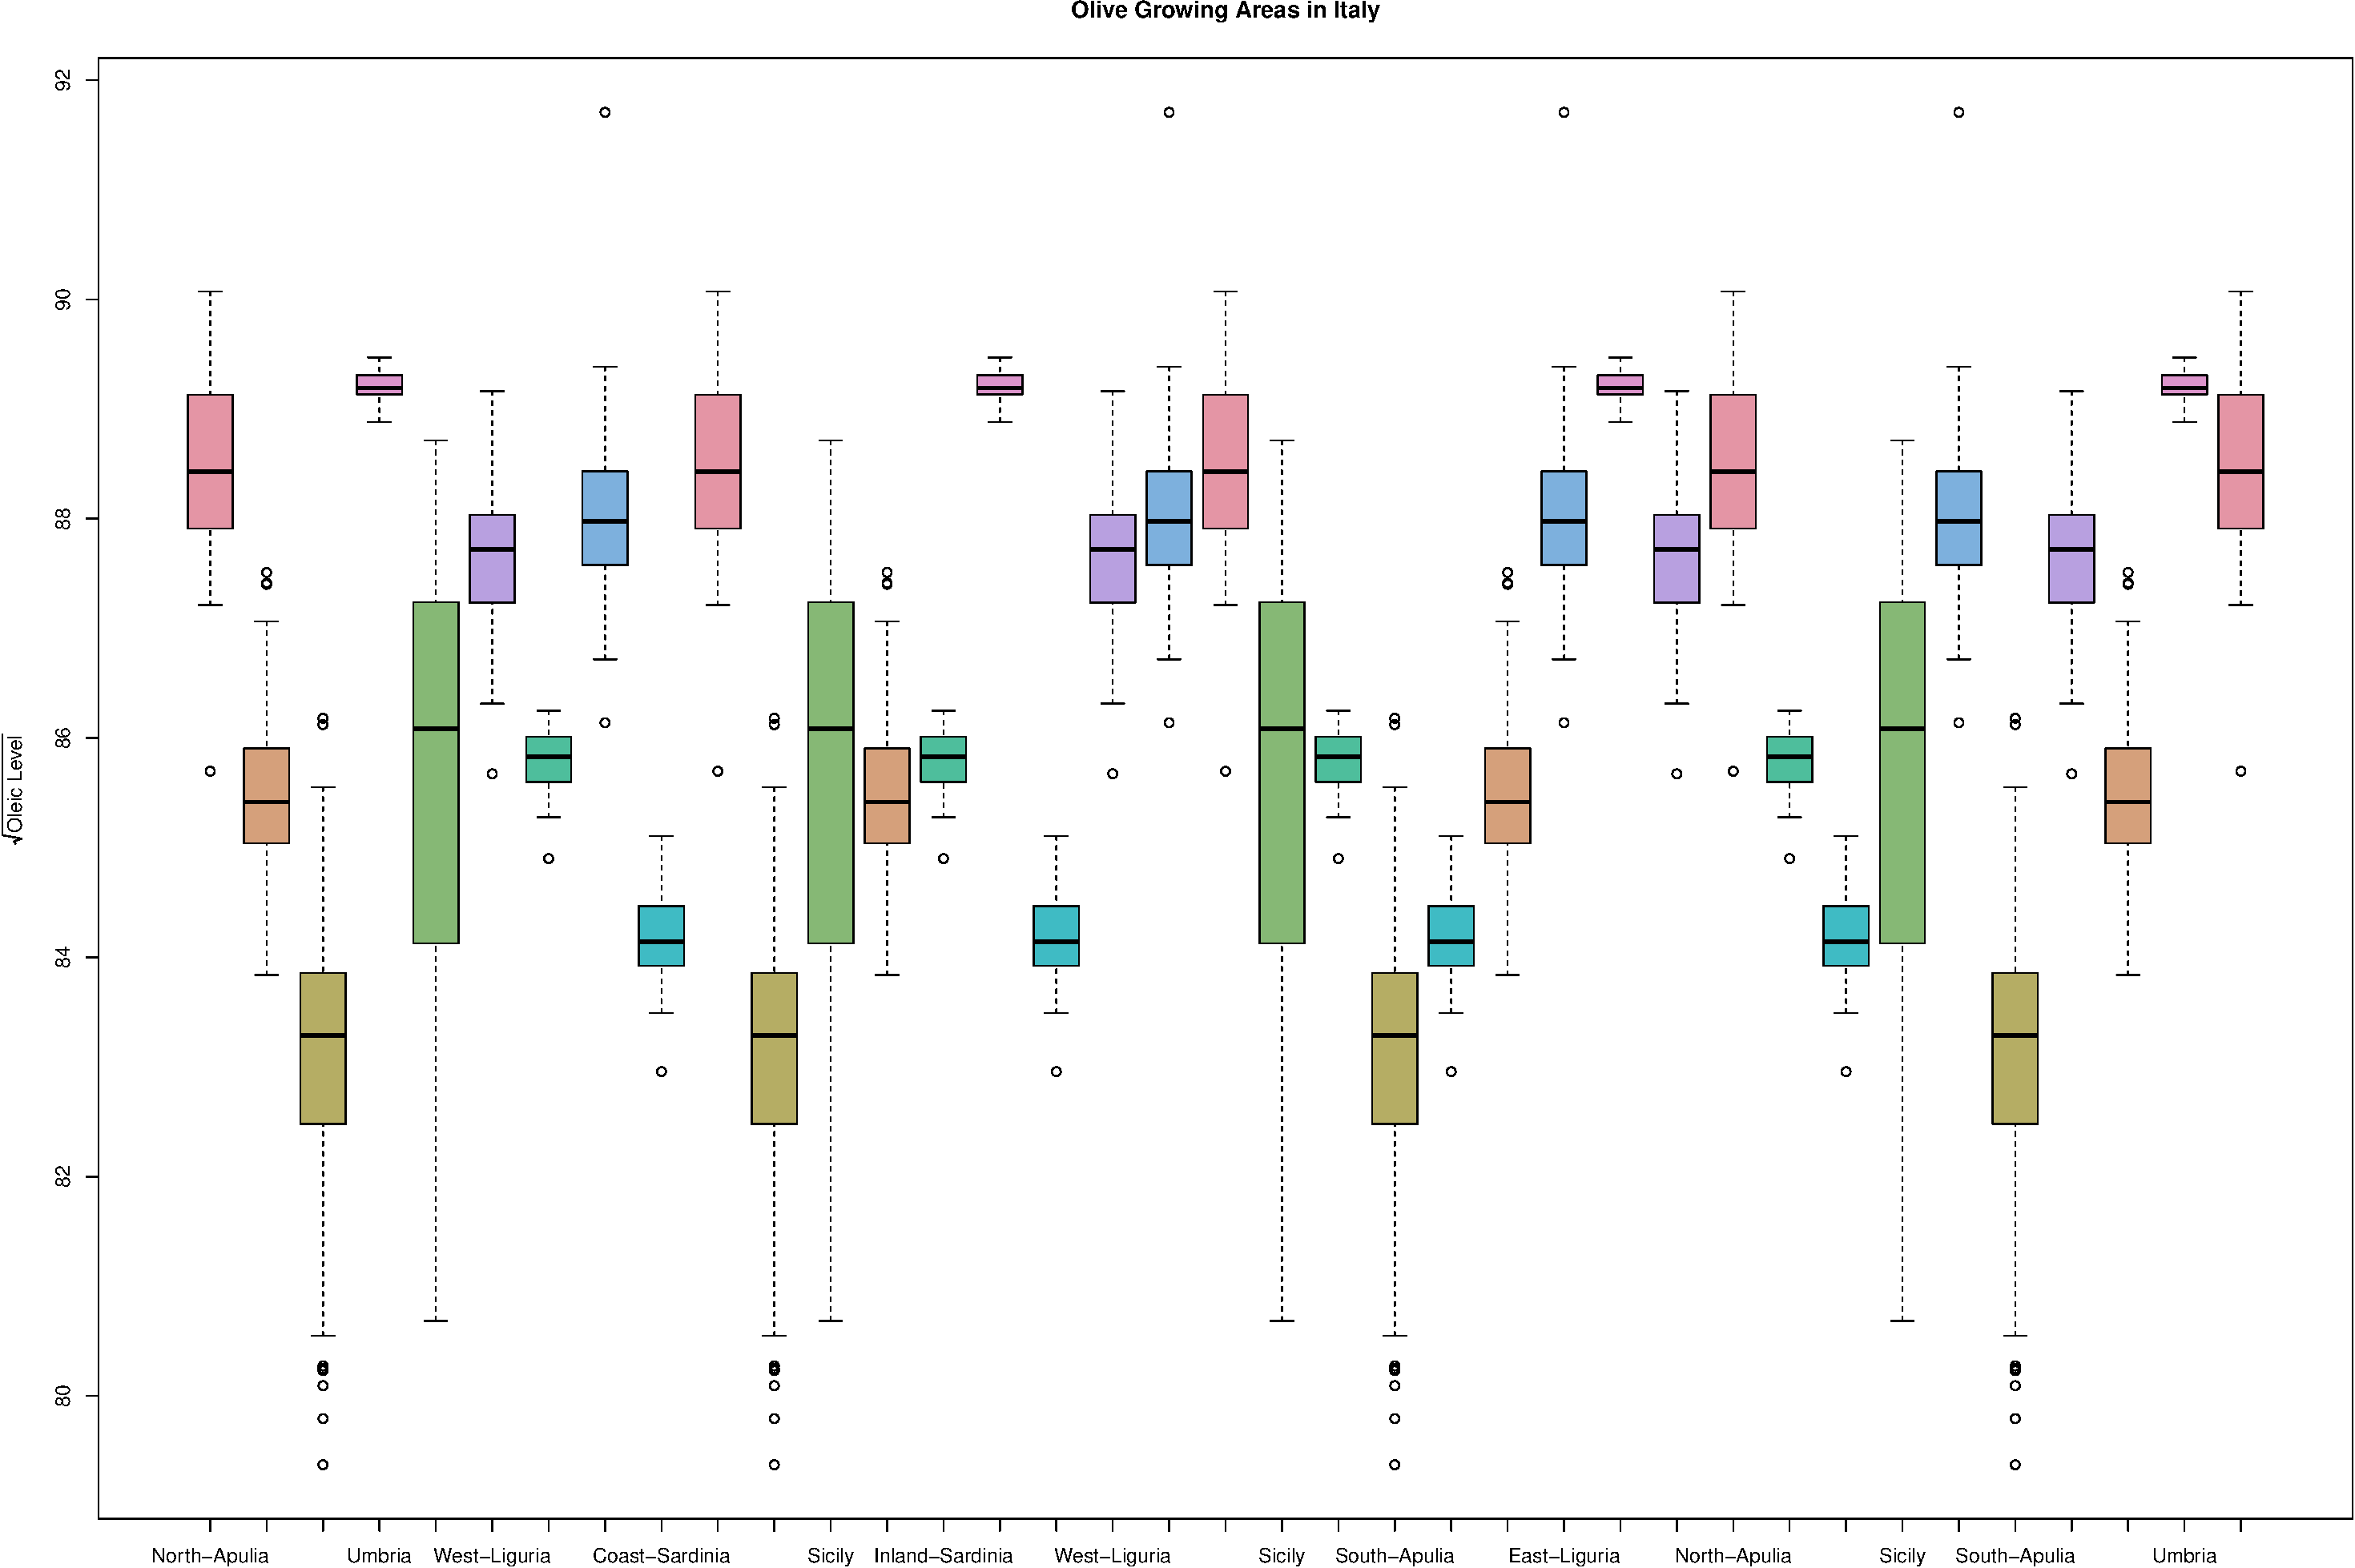
\includegraphics{a4_solutions_files/figure-latex/unnamed-chunk-15-1} \end{center}

\eitem

\item 

(7 marks) Construct \(t\) tests for every pair of olive growing areas
(recall \texttt{pairwise.t.test} from class). Use the significance
levels from these tests to construct an ordering of the boxplot pairs,
one which favours having the most significantly different pairs at the
left of the display. \bitem
\item Show your code. \item Show the resulting display.

\begin{Shaded}
\begin{Highlighting}[]
\CommentTok{# running the pairwise t-tests}
\NormalTok{t_tests =}\StringTok{ }\KeywordTok{with}\NormalTok{(olive,}
               \KeywordTok{pairwise.t.test}\NormalTok{(}\KeywordTok{sqrt}\NormalTok{(oleic), Area))}

\CommentTok{# creating a matrix of weights set to the sig. levels of the t-tests}
\NormalTok{weights =}\StringTok{ }\KeywordTok{matrix}\NormalTok{(}\DecValTok{0}\NormalTok{, }\DataTypeTok{nrow=}\NormalTok{n, }\DataTypeTok{ncol=}\NormalTok{n)}
\KeywordTok{rownames}\NormalTok{(weights) =}\StringTok{ }\KeywordTok{names}\NormalTok{(groups)}
\KeywordTok{colnames}\NormalTok{(weights) =}\StringTok{ }\KeywordTok{names}\NormalTok{(groups)}
\NormalTok{weights[}\DecValTok{2}\OperatorTok{:}\NormalTok{n, }\DecValTok{1}\OperatorTok{:}\NormalTok{(n}\OperatorTok{-}\DecValTok{1}\NormalTok{)] =}\StringTok{ }\NormalTok{t_tests}\OperatorTok{$}\NormalTok{p.value}

\CommentTok{# getting rid of the NA values and fixing the weights matrix}
\KeywordTok{diag}\NormalTok{(weights) =}\StringTok{ }\DecValTok{0}
\ControlFlowTok{for}\NormalTok{(i }\ControlFlowTok{in} \DecValTok{1}\OperatorTok{:}\NormalTok{(n}\OperatorTok{-}\DecValTok{1}\NormalTok{)) \{}
  \ControlFlowTok{for}\NormalTok{(j }\ControlFlowTok{in}\NormalTok{ (i}\OperatorTok{+}\DecValTok{1}\NormalTok{)}\OperatorTok{:}\NormalTok{n) \{}
\NormalTok{    weights[i,j] =}\StringTok{ }\NormalTok{weights[j,i]}
\NormalTok{  \}}
\NormalTok{\}}

\NormalTok{highlowEulOrd =}\StringTok{ }\KeywordTok{eulerian}\NormalTok{(}\OperatorTok{-}\NormalTok{weights)}
\KeywordTok{boxplot}\NormalTok{(groups[highlowEulOrd], }\DataTypeTok{col=}\NormalTok{cols[highlowEulOrd],}
        \DataTypeTok{ylab=}\KeywordTok{expression}\NormalTok{(}\KeywordTok{sqrt}\NormalTok{(}\StringTok{"Oleic Level"}\NormalTok{)),}
        \DataTypeTok{main=}\StringTok{"Olive Growing Areas in Italy"}\NormalTok{)}
\end{Highlighting}
\end{Shaded}

\begin{center}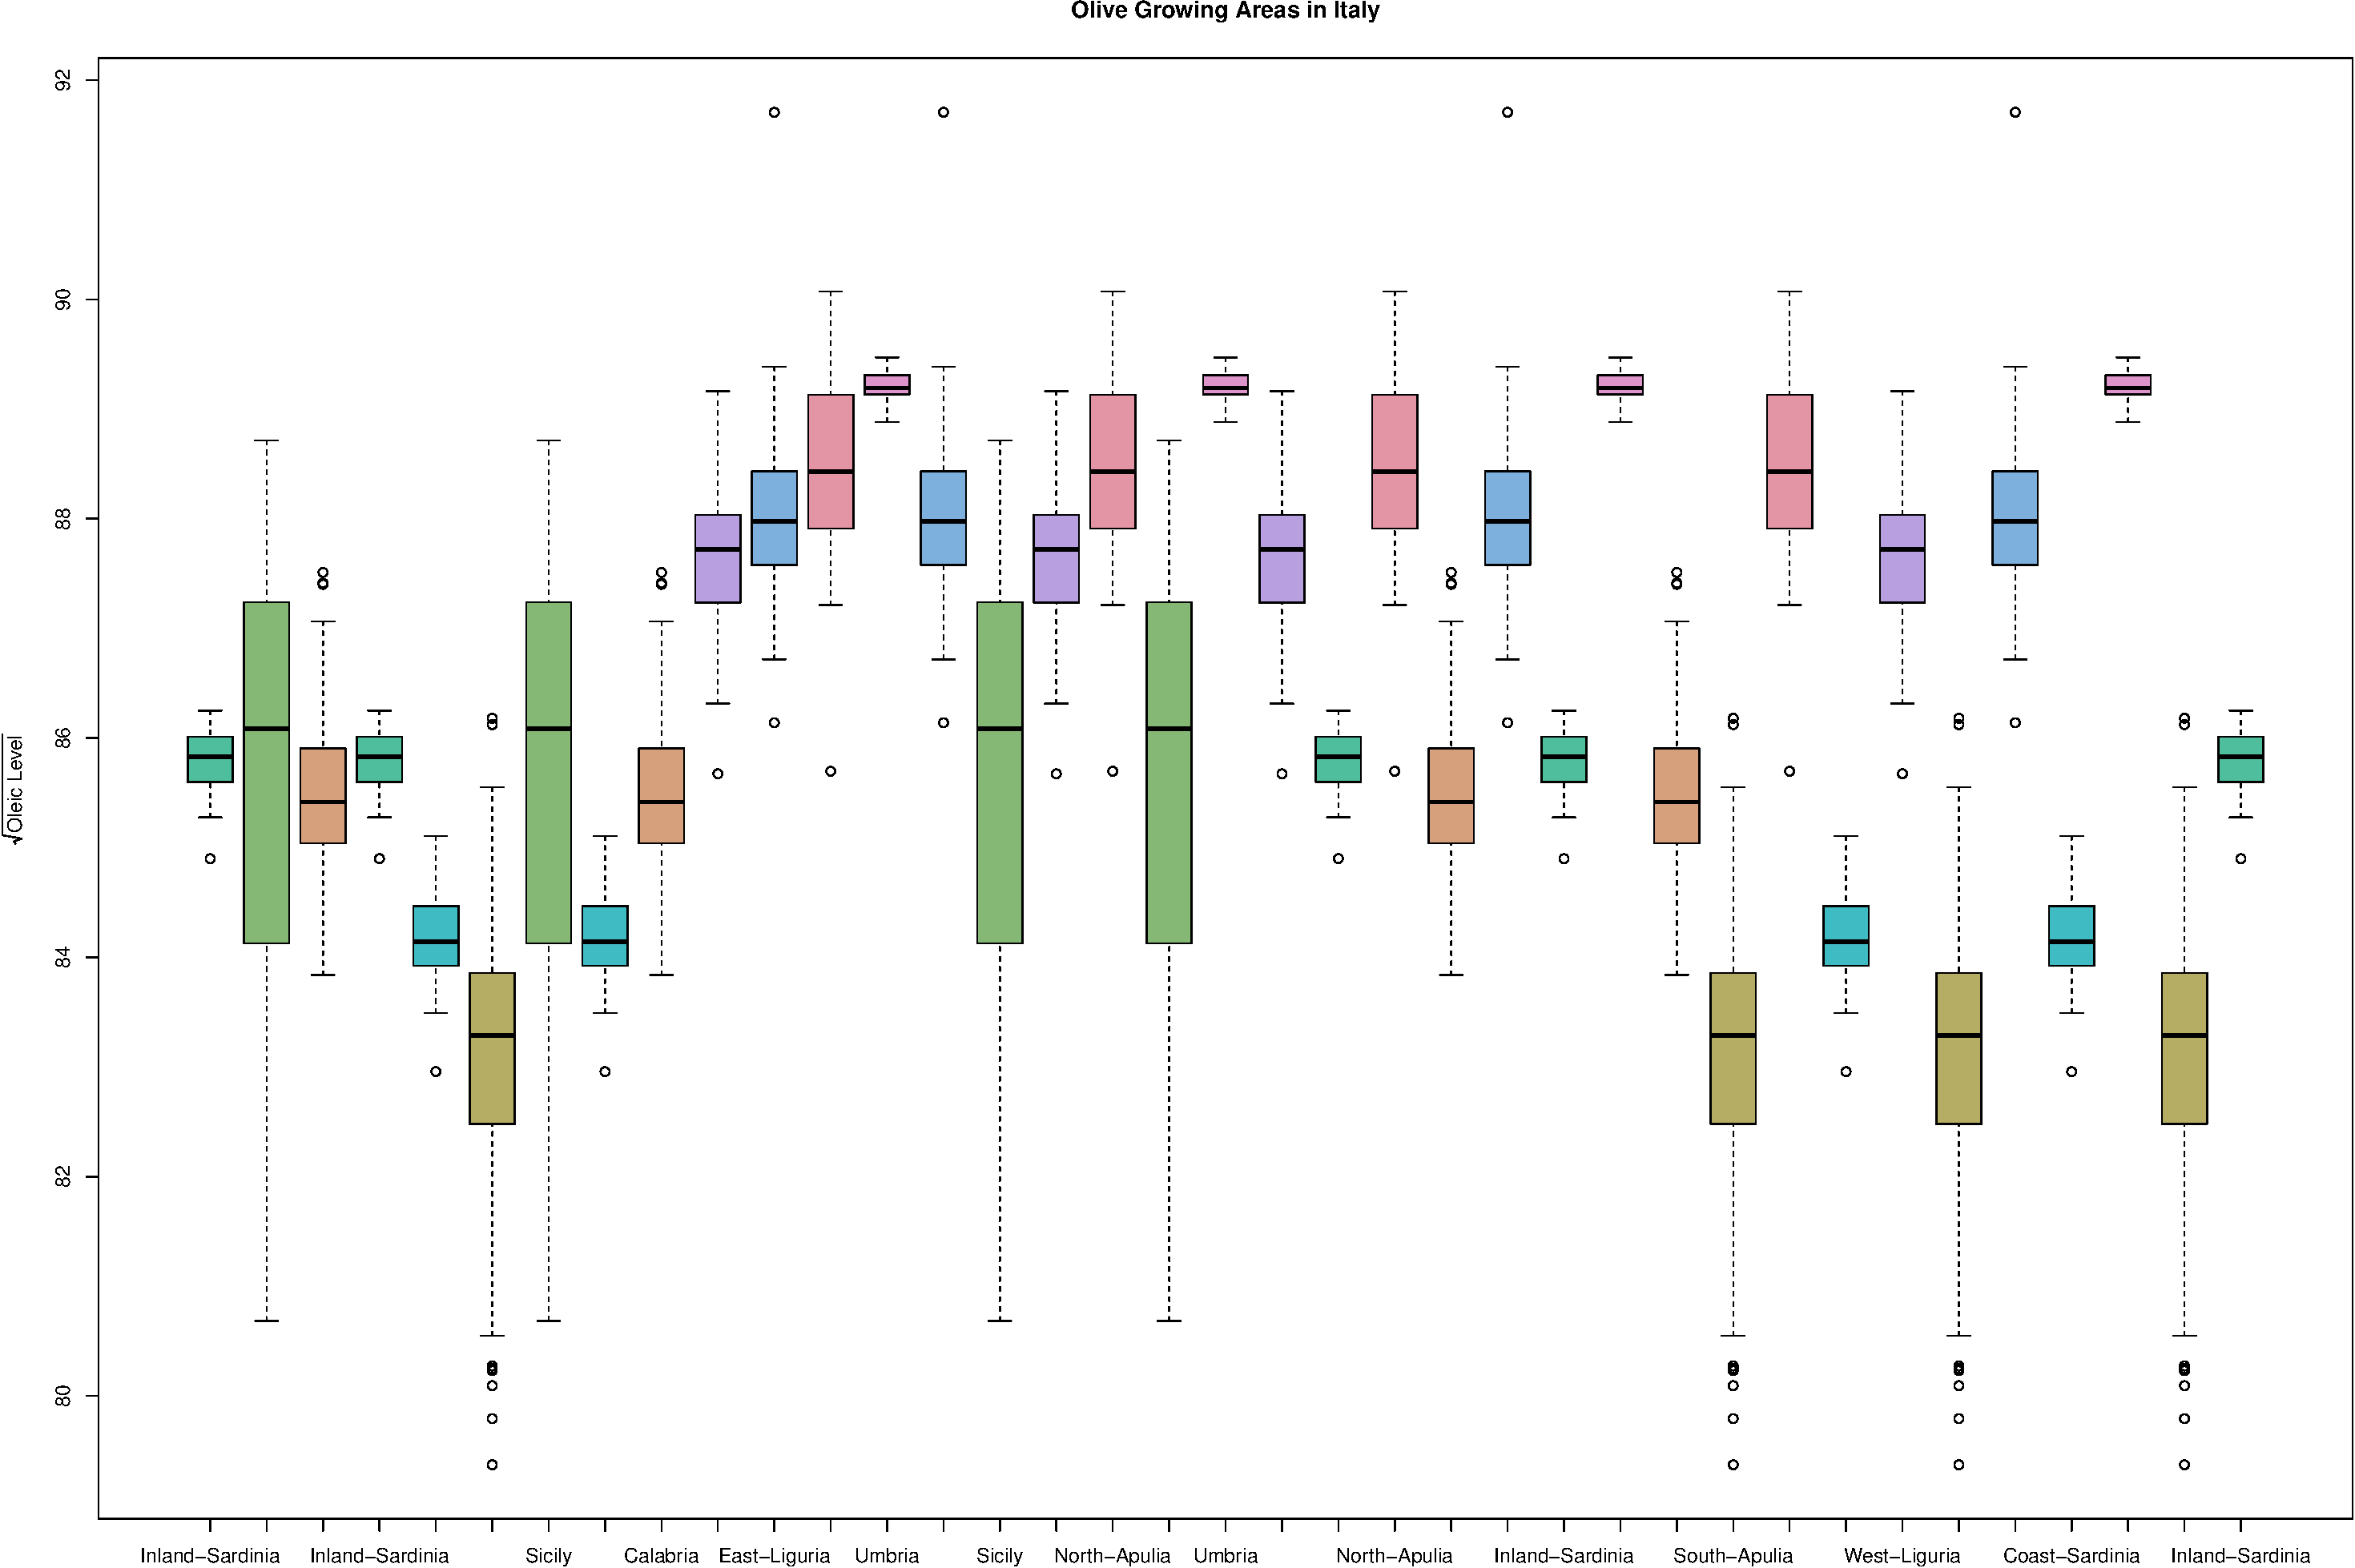
\includegraphics{a4_solutions_files/figure-latex/unnamed-chunk-16-1} \end{center}

\item 

Does the ordering perfectly arrange the boxplots so that for any
pairwise comparison, those to the left are more significant and those to
the right are less significant?

No. The majority of the medians of the boxplots pairs get closer in
value, i.e more identical, as the diagram moves from left to right, and
the pairs become easier to compare as a result because the boxplots
become more in line with each other on the vertical scale. So most of
the pairwise comparisons are ordered correctly. However, some of them
(e.g.~the comparison between Sicily and Coast-Sardinia) are less
significant than the comparisons to their right, and should be located
further to the right of the plot.

\item 

Explain why the ordering was successful (or unsuccessful) in this way.

This is likely because a Eulerian path cannot have an edges walked
through again. Hence, once the Eulerian has traversed an edge and
arrived at a node/region, it will choose to take the next shortest path
possible from that node and it cannot travel through edges it has
already visited to get to the a different path. Hence, when creating the
ordering for the boxplots, the next comparison is determined by the next
most significant pairwise comparison for the node that is currently
being visited, and this may not always which may not be necessarily the
next most significant pairwise comparison overall.

\item 

Show a display showing only the first 8 comparisons.

\begin{Shaded}
\begin{Highlighting}[]
\NormalTok{mostSig8 =}\StringTok{ }\NormalTok{highlowEulOrd[}\DecValTok{1}\OperatorTok{:}\DecValTok{9}\NormalTok{]}

\KeywordTok{boxplot}\NormalTok{(groups[mostSig8], }
        \DataTypeTok{col=}\NormalTok{cols[mostSig8],}
        \DataTypeTok{ylab=}\KeywordTok{expression}\NormalTok{(}\KeywordTok{sqrt}\NormalTok{(}\StringTok{"Oleic Level"}\NormalTok{)),}
        \DataTypeTok{main=}\StringTok{"Olive Growing Areas in Italy"}\NormalTok{)}
\end{Highlighting}
\end{Shaded}

\begin{center}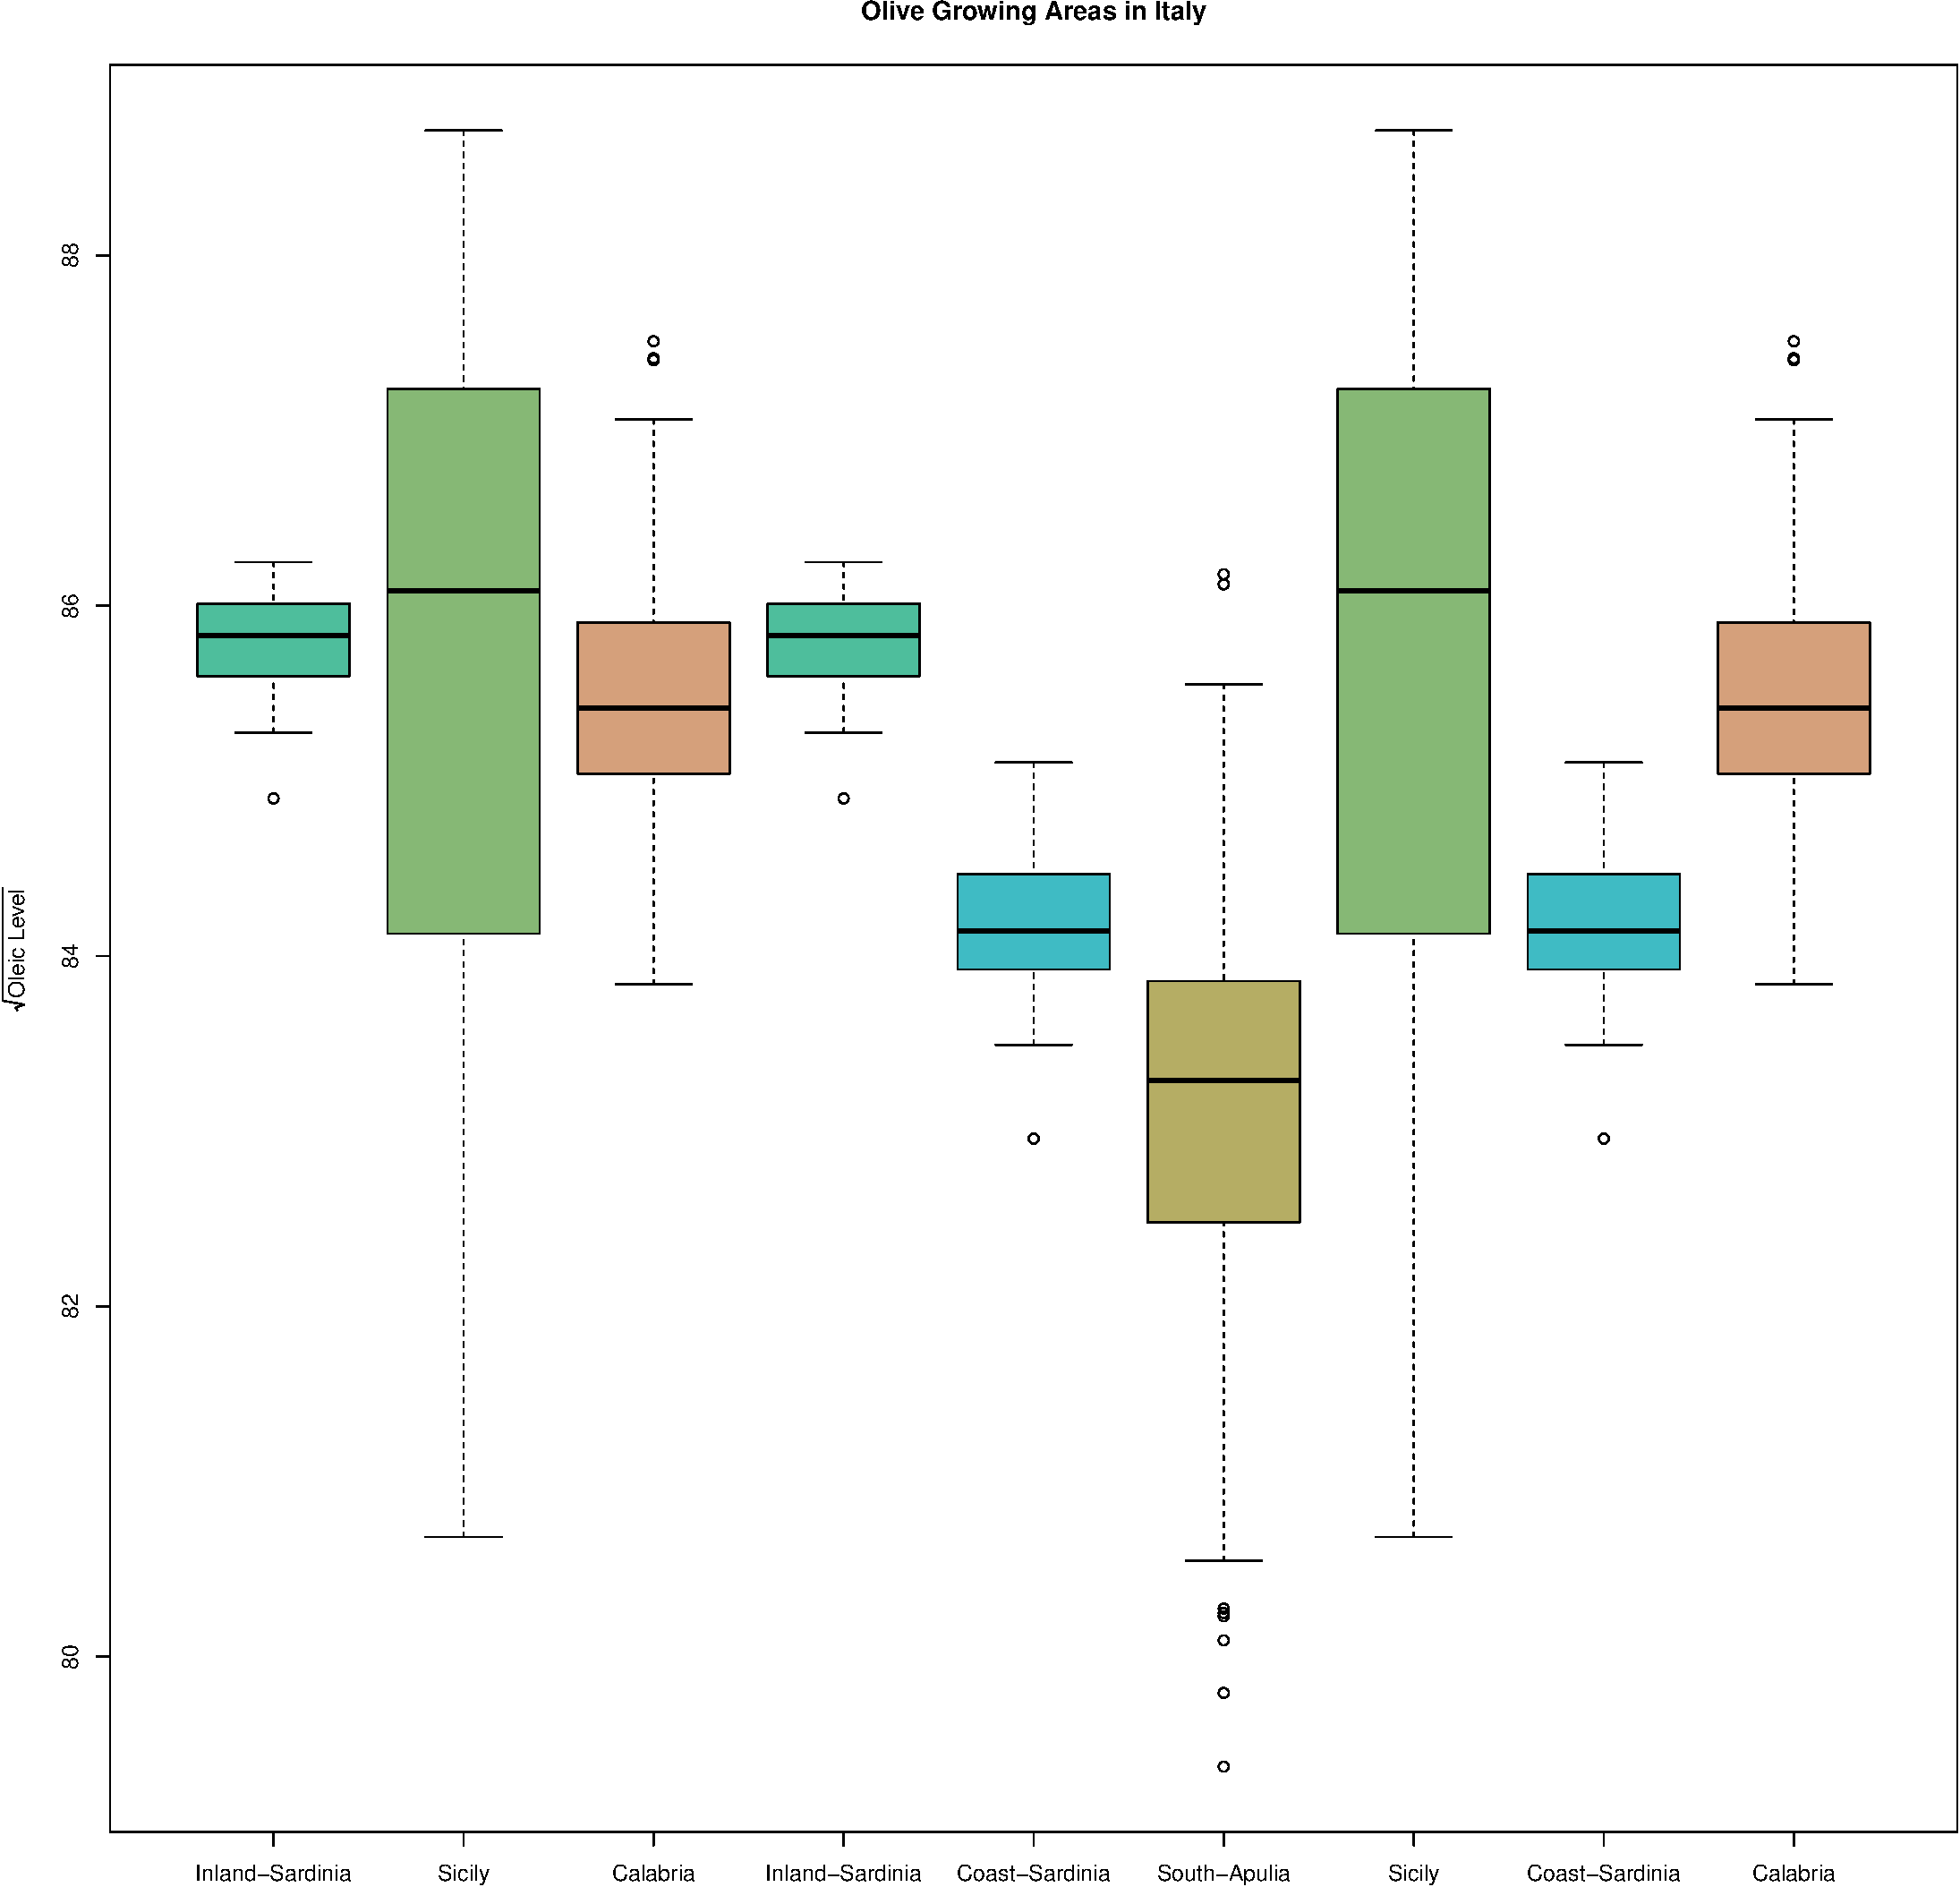
\includegraphics{a4_solutions_files/figure-latex/unnamed-chunk-17-1} \end{center}

\eitem

\item 

(7 marks) Use the significance levels from part (iii) but now order the
boxplots so that the \textbf{least} significant differences appear
earliest in the sequence from left to right. \bitem
\item Show your code. \item Show the resulting display.

\begin{Shaded}
\begin{Highlighting}[]
\NormalTok{lowhighEulOrd =}\StringTok{ }\KeywordTok{eulerian}\NormalTok{(weights)}
\KeywordTok{boxplot}\NormalTok{(groups[lowhighEulOrd], }\DataTypeTok{col=}\NormalTok{cols[lowhighEulOrd],}
        \DataTypeTok{ylab=}\KeywordTok{expression}\NormalTok{(}\KeywordTok{sqrt}\NormalTok{(}\StringTok{"Oleic Level"}\NormalTok{)),}
        \DataTypeTok{main=}\StringTok{"Oleic Levels by Olive Growing Area"}\NormalTok{)}
\end{Highlighting}
\end{Shaded}

\begin{center}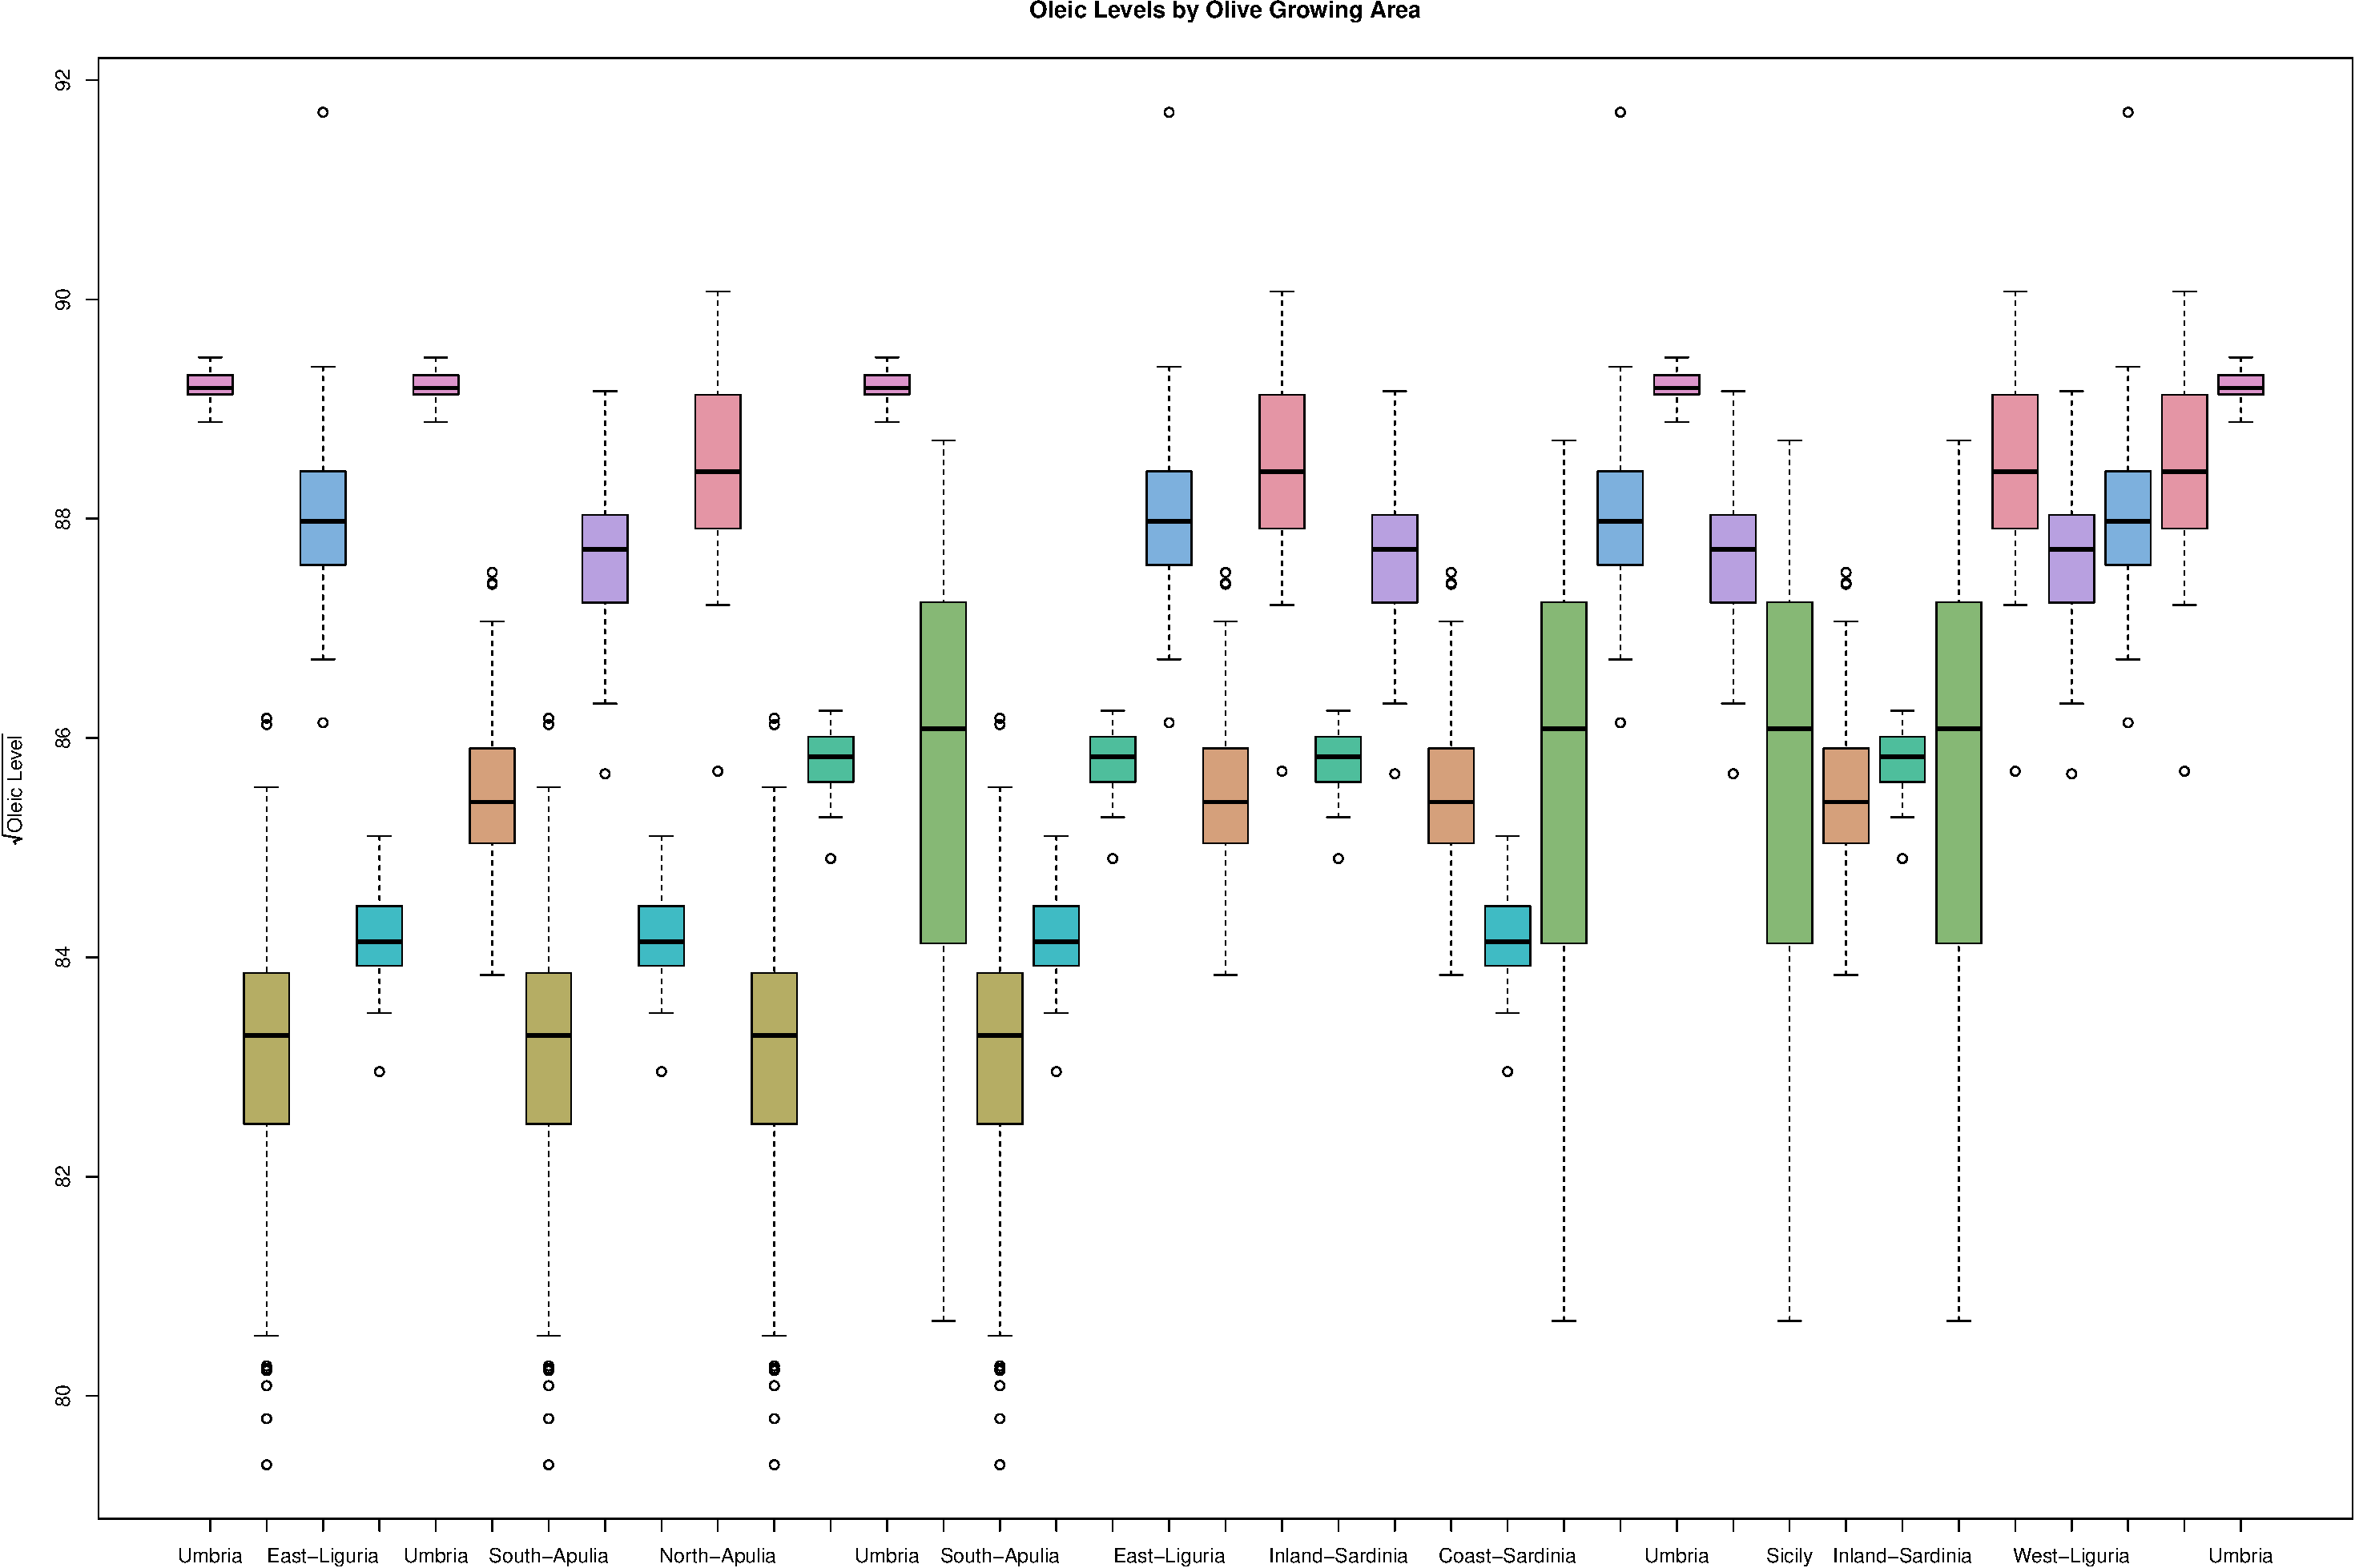
\includegraphics{a4_solutions_files/figure-latex/unnamed-chunk-18-1} \end{center}

\item 

Does the ordering perfectly arrange the boxplots so that for any
pairwise comparison, those to the left are less significant and those to
the right are more significant?

No. For the most part, the medians of the boxplots pairs get further
away in value, i.e less identical, as the diagram moves from left to
right, and the pairs become more to compare as a result because the
boxplots become more out of line with each other on the vertical scale.
So most of the pairwise comparisons are ordered correctly. However, some
of them (e.g.~the comparison between South-Apulia and Coast-Sardinia)
are more significant than the comparisons to their right, and should be
located further to the right of the plot.

\item 

Explain why the ordering was successful (or unsuccessful) in this way.

This was unsuccessful for the same reasons as mentioned in the previous
question: since the algorithm for \texttt{eulerian} is greedy and an
edge that has already been traversed cannot be visited again, the next
comparison is determined by the next least significant pairwise
comparison for the node/region that is currently being visited, and this
may not always which may not be necessarily the next least significant
pairwise comparison overall.

\item 

Show a display showing only the first 8 comparisons.

\begin{Shaded}
\begin{Highlighting}[]
\NormalTok{leastSig8 =}\StringTok{ }\NormalTok{lowhighEulOrd[}\DecValTok{1}\OperatorTok{:}\DecValTok{9}\NormalTok{]}

\KeywordTok{boxplot}\NormalTok{(groups[leastSig8], }
        \DataTypeTok{col=}\NormalTok{cols[leastSig8],}
        \DataTypeTok{ylab=}\KeywordTok{expression}\NormalTok{(}\KeywordTok{sqrt}\NormalTok{(}\StringTok{"Oleic Level"}\NormalTok{)),}
        \DataTypeTok{main=}\StringTok{"Olive Growing Areas in Italy"}\NormalTok{)}
\end{Highlighting}
\end{Shaded}

\begin{center}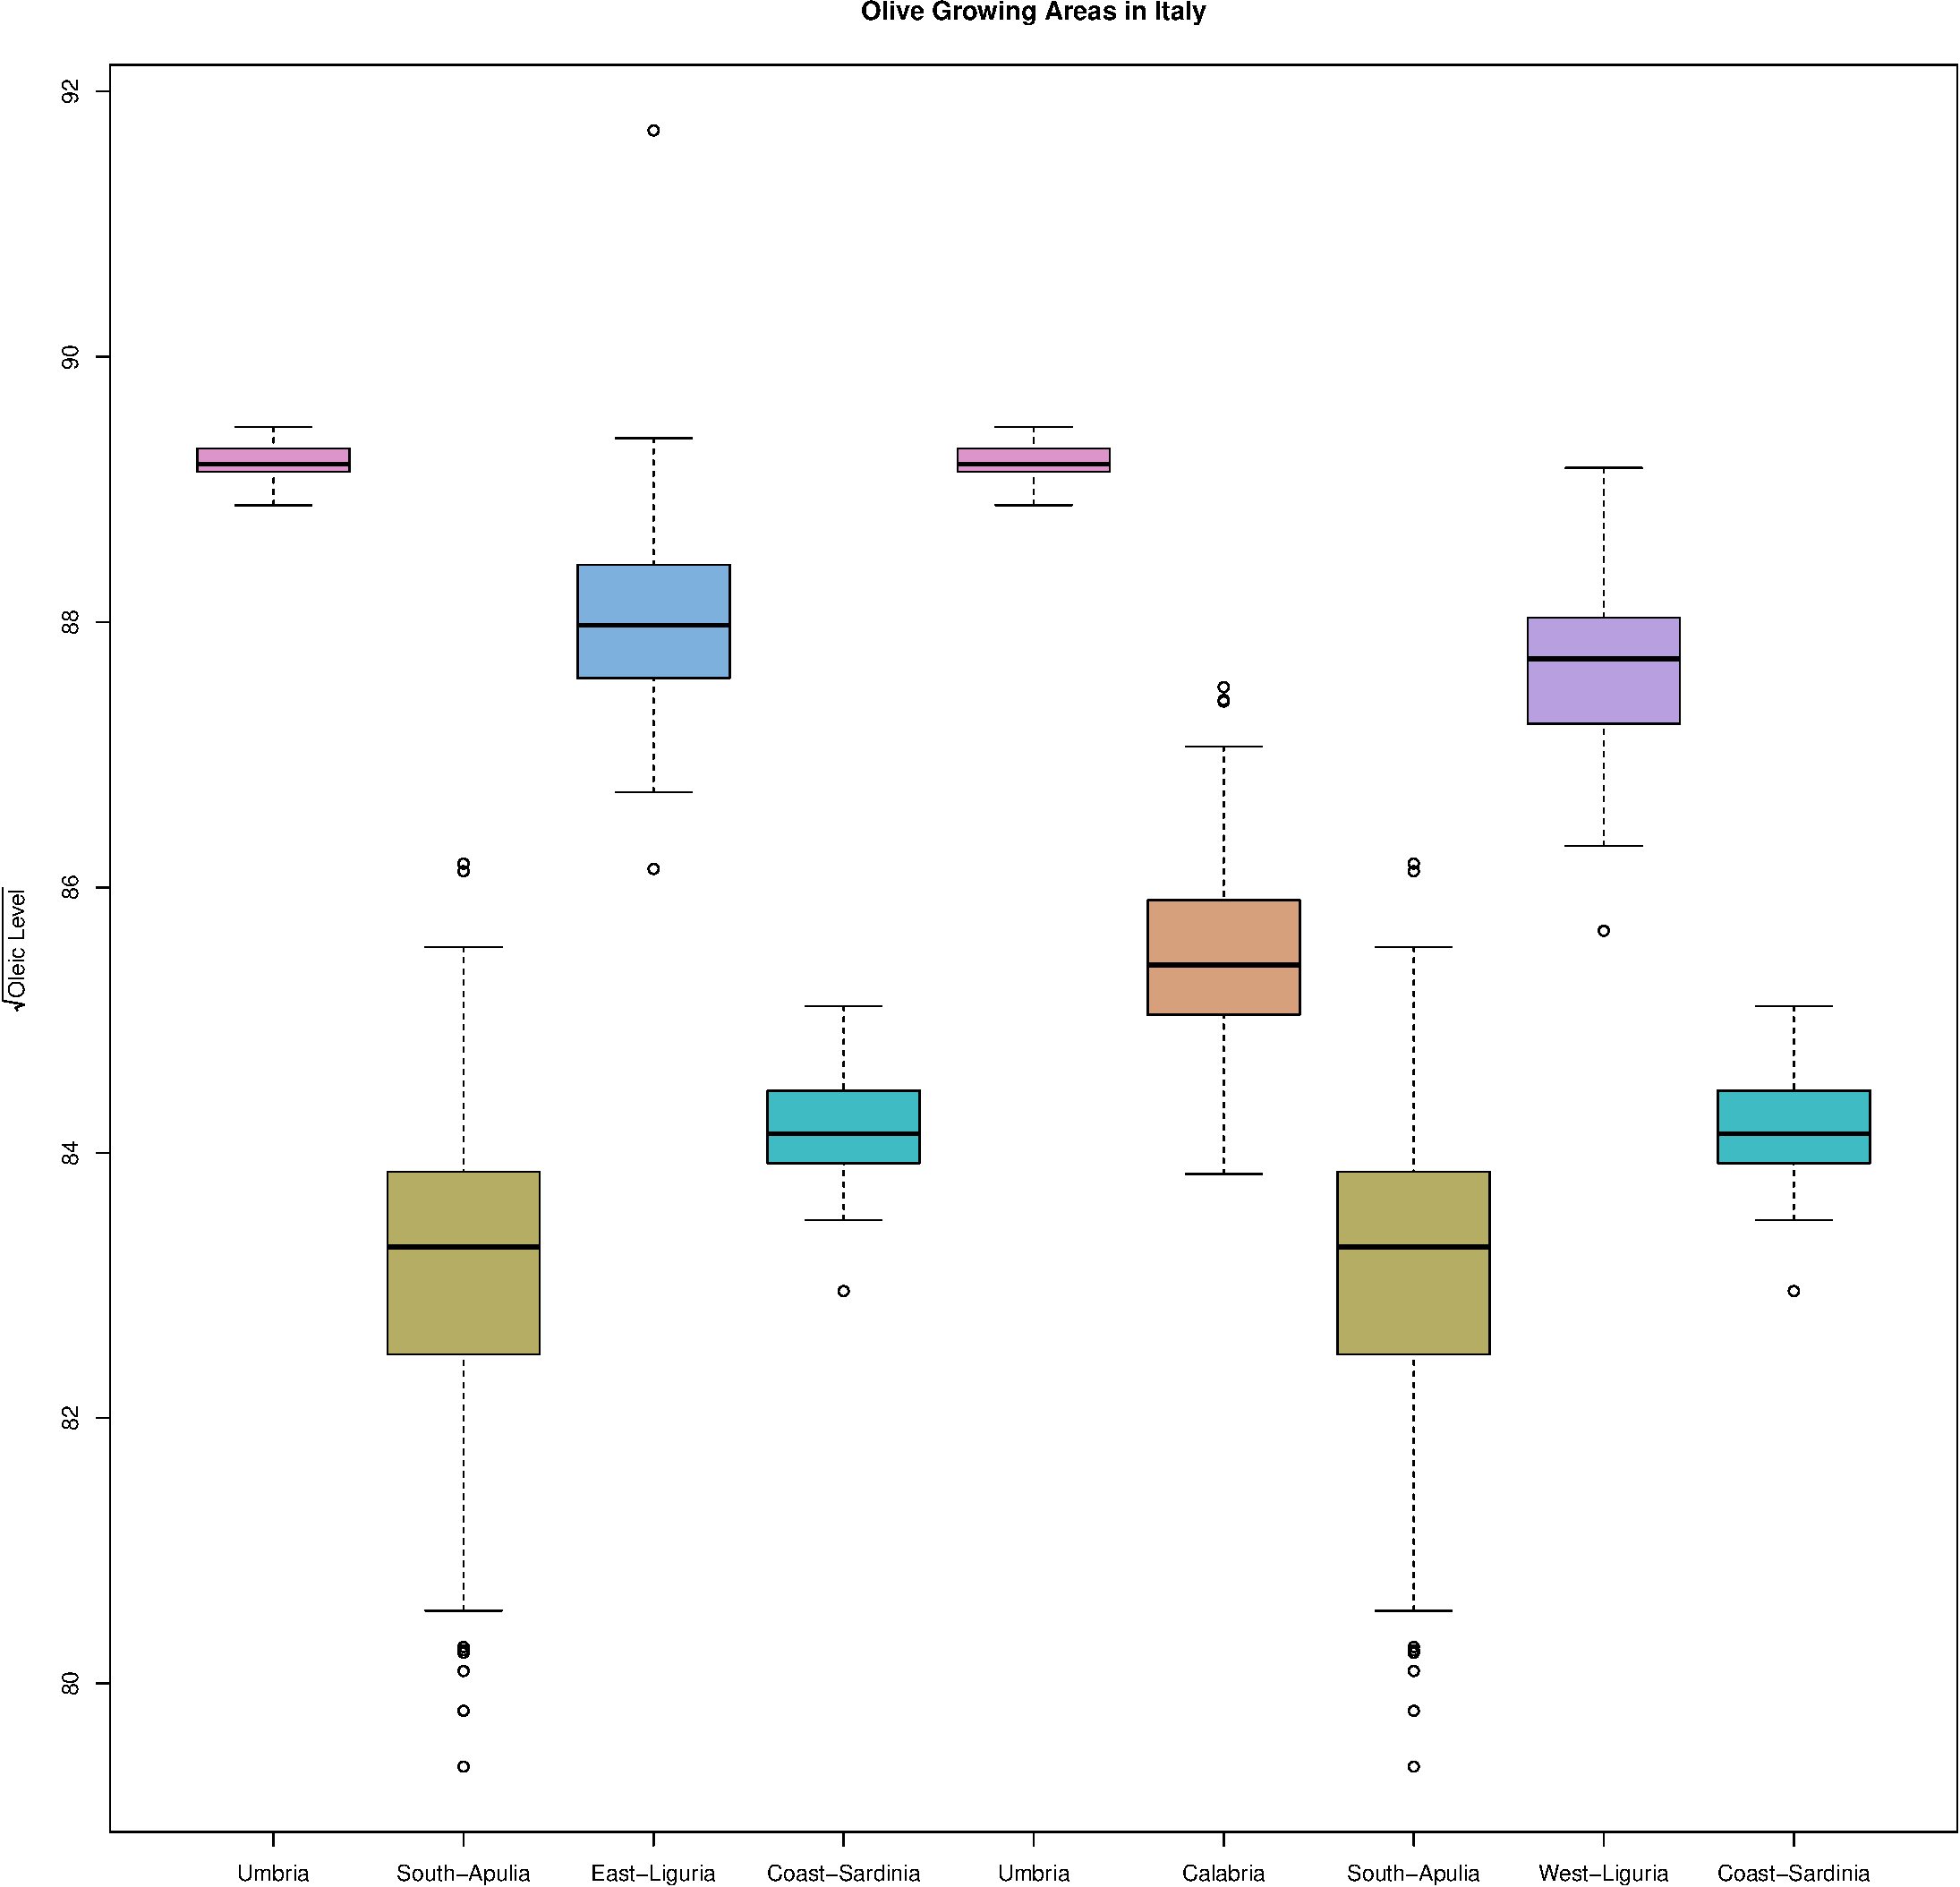
\includegraphics{a4_solutions_files/figure-latex/unnamed-chunk-19-1} \end{center}

\eitem

\item 

(2 marks) Is the sequence used in part (iii) the reverse of that in part
(iv)?

No, it is not.

\bitem
\item If it is, must it be the reverse?

No, it doesn't because there are 36 unique pairwise comparisons that can
be made, so the the set of the 8 most significant ones and the set of
the 8 least signifcant ones (but in reverse order) will not be the same,
i.e.~will not fully overlap, as this could only happen if the Eulerian
traversed the same edges again, which by definition does not occur.

\item 

If it is not, is it impossible for it to be the same?

For this type of comparison, it is possible.

\item 

Either way, explain your reasoning.

Note that the plots of all the comparisons from most significant to
least is the reverse of the plots from least to most. Hence, the only
way that it would be possible for part (iii) to be the reverse of part
(iv) is if there were only 8 pairwise comparisons in total to consider,
instead of 36.

\eitem

\eenum

\item 

The olive growing areas are divided into three different regions: North,
South, and Sardinia. In this part of the question, interest lies only in
comparisons between each growing area in the south and each area in
Sardinia. That is, each southern area (4 areas) is to be compared to
each Sardinian area (2 areas) yielding a total of 8 comparisons of
interest.

\benum
\item (4 marks) Having loaded \texttt{PairViz}, create a graph having
all six areas in the South and Sardinia as nodes and with edges between
every pair whose comparison is of interest. \bitem
\item plot this graph \item show the code used to create the graph and
to plot it.

\begin{Shaded}
\begin{Highlighting}[]
\NormalTok{regional =}\StringTok{ }\NormalTok{olive[olive}\OperatorTok{$}\NormalTok{Region }\OperatorTok\StringTok{ }\KeywordTok{c}\NormalTok{(}\StringTok{'South'}\NormalTok{,}\StringTok{'Sardinia'}\NormalTok{),]}
\NormalTok{regions =}\StringTok{ }\KeywordTok{with}\NormalTok{(regional, }\KeywordTok{split}\NormalTok{(}\KeywordTok{sqrt}\NormalTok{(oleic), }\KeywordTok{list}\NormalTok{(Area,Region), }\DataTypeTok{drop=}\OtherTok{TRUE}\NormalTok{))}
\NormalTok{nodes =}\StringTok{ }\KeywordTok{names}\NormalTok{(regions)}
\NormalTok{SouthRegions =}\StringTok{ }\NormalTok{nodes[}\KeywordTok{endsWith}\NormalTok{(nodes, }\StringTok{"South"}\NormalTok{)]}
\NormalTok{SardiniaRegions =}\StringTok{ }\NormalTok{nodes[}\OperatorTok{!}\KeywordTok{endsWith}\NormalTok{(nodes, }\StringTok{"South"}\NormalTok{)]}
\NormalTok{RegionGraph =}\StringTok{ }\KeywordTok{new}\NormalTok{(}\StringTok{"graphNEL"}\NormalTok{, }\DataTypeTok{nodes=}\NormalTok{nodes, }\DataTypeTok{edgemode=}\StringTok{"undirected"}\NormalTok{)}
\ControlFlowTok{for}\NormalTok{ (i }\ControlFlowTok{in} \DecValTok{1}\OperatorTok{:}\DecValTok{4}\NormalTok{) \{}
\NormalTok{  stregion =}\StringTok{ }\NormalTok{SouthRegions[i]}
  \ControlFlowTok{for}\NormalTok{ (j }\ControlFlowTok{in} \DecValTok{1}\OperatorTok{:}\DecValTok{2}\NormalTok{) \{}
\NormalTok{    sdregion =}\StringTok{ }\NormalTok{SardiniaRegions[j]}
\NormalTok{    RegionGraph =}\StringTok{ }\KeywordTok{addEdge}\NormalTok{(stregion, sdregion, RegionGraph)}
\NormalTok{  \}}
\NormalTok{\}}

\KeywordTok{plot}\NormalTok{(RegionGraph, }\StringTok{"circo"}\NormalTok{)}
\end{Highlighting}
\end{Shaded}

\begin{center}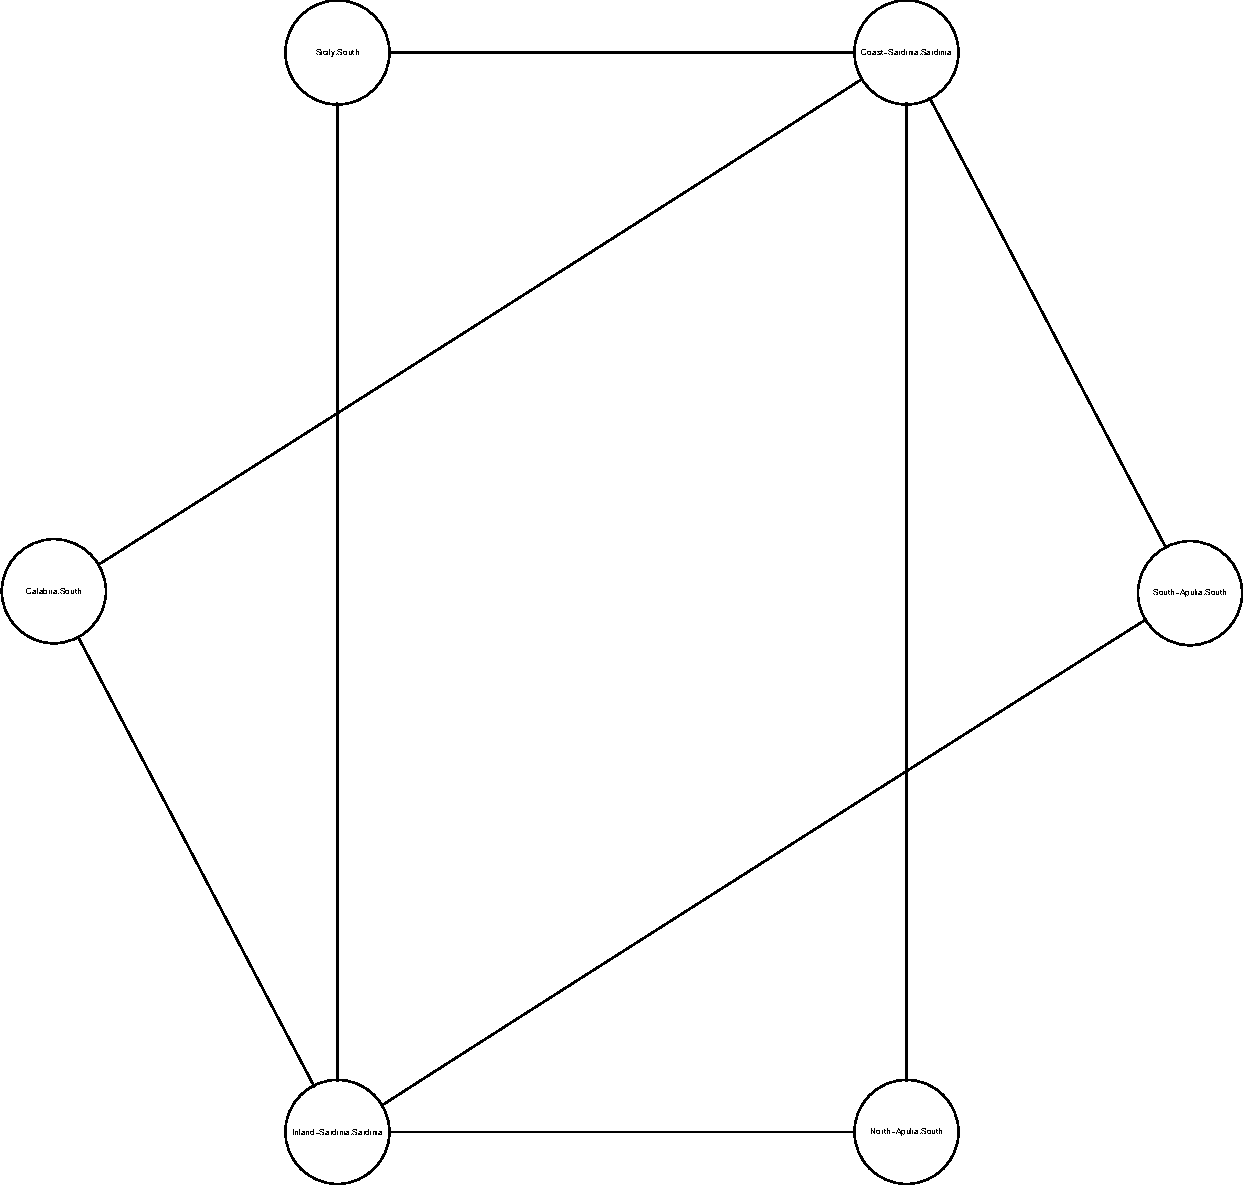
\includegraphics{a4_solutions_files/figure-latex/unnamed-chunk-20-1} \end{center}

\eitem

\item 

(4 marks) Using the graph from part (i), construct an Eulerian and use
that Eulerian to produce a sequence of boxplots that show the
comparisons of interest. \bitem
\item show the boxplot display \item show the code used to construct the
Eulerian and the display.

\begin{Shaded}
\begin{Highlighting}[]
\NormalTok{ssOrd =}\StringTok{ }\KeywordTok{eulerian}\NormalTok{(RegionGraph)}

\NormalTok{colEulOrd =}\StringTok{ }\KeywordTok{rep}\NormalTok{(}\DecValTok{0}\NormalTok{, }\KeywordTok{length}\NormalTok{(ssOrd))}
\ControlFlowTok{for}\NormalTok{ (i }\ControlFlowTok{in} \DecValTok{1}\OperatorTok{:}\KeywordTok{length}\NormalTok{(ssOrd)) \{}
\NormalTok{  colEulOrd[i] =}\StringTok{  }\KeywordTok{which}\NormalTok{(nodes}\OperatorTok{==}\NormalTok{ssOrd[i])}
\NormalTok{\}}

\KeywordTok{boxplot}\NormalTok{(regions[ssOrd], }\DataTypeTok{col=}\NormalTok{cols[colEulOrd],}
        \DataTypeTok{ylab=}\KeywordTok{expression}\NormalTok{(}\KeywordTok{sqrt}\NormalTok{(}\StringTok{"Oleic Level"}\NormalTok{)),}
        \DataTypeTok{main=}\StringTok{"Olive Growing Areas in the South and Sardinia"}\NormalTok{)}
\end{Highlighting}
\end{Shaded}

\begin{center}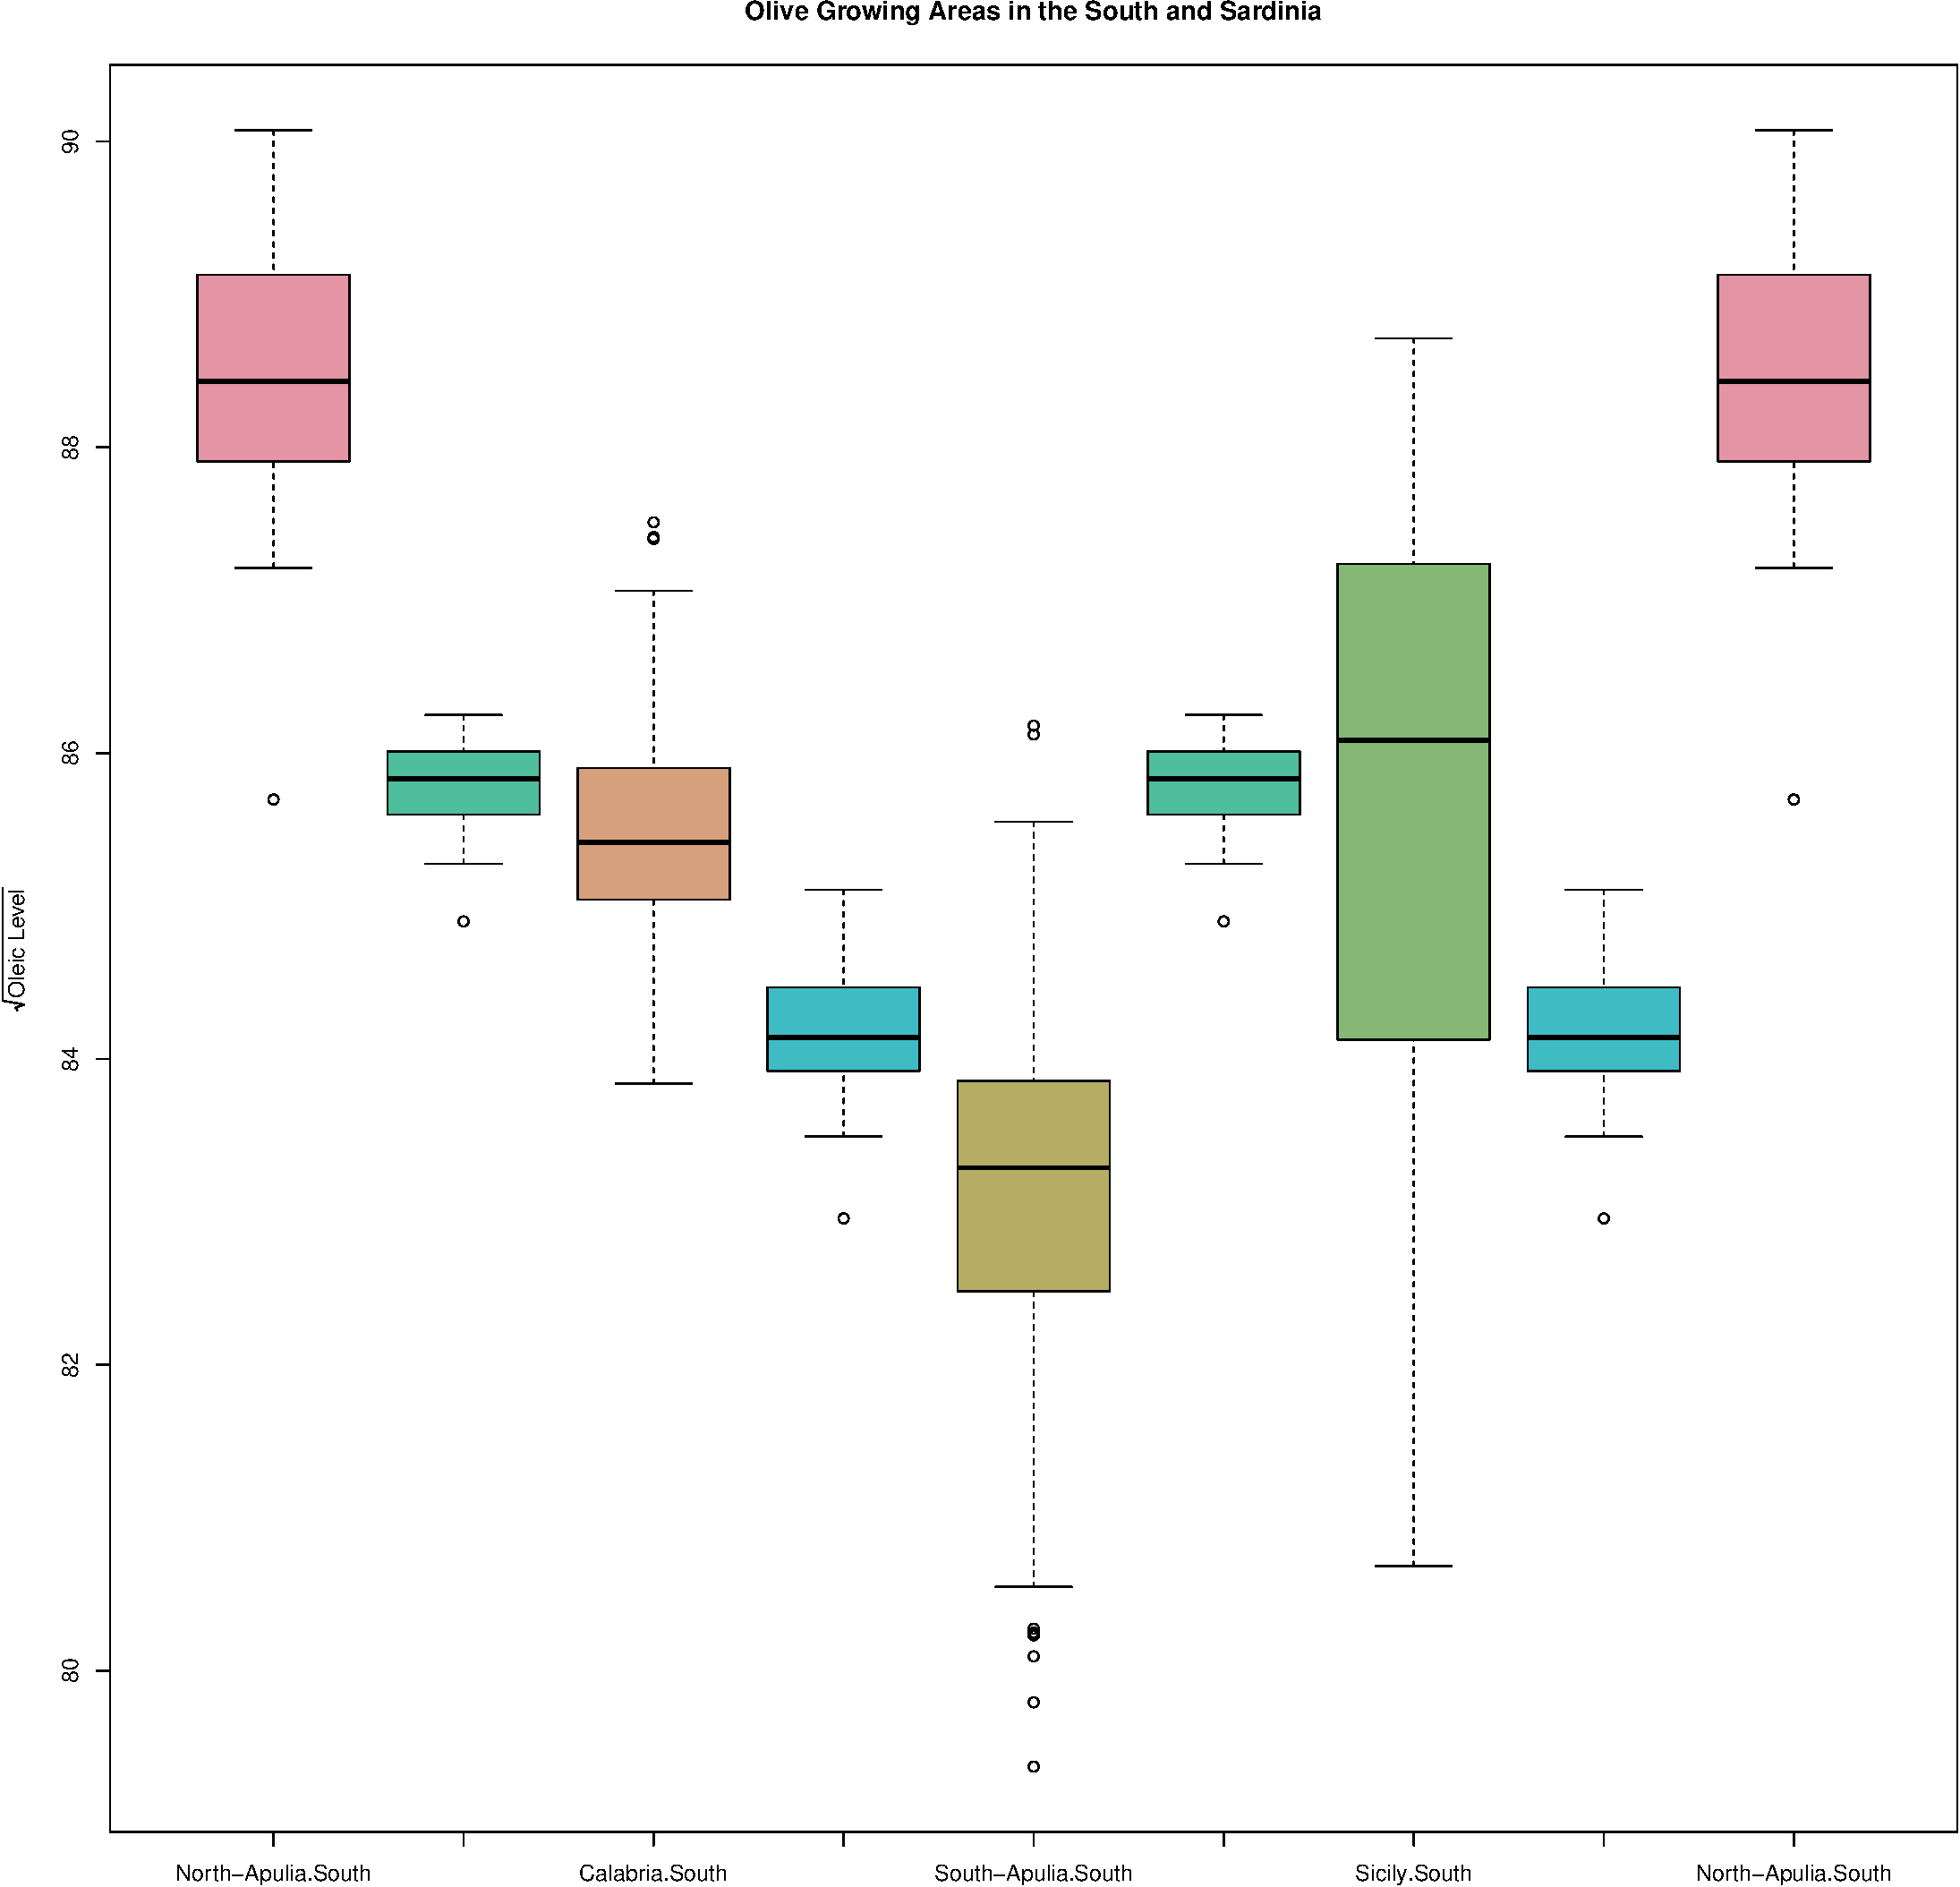
\includegraphics{a4_solutions_files/figure-latex/unnamed-chunk-21-1} \end{center}

\eitem

\eenum
\eenum

\item  

\textbf{Antarctic sea ice} On the website for this assignment, in the
directory called \texttt{R} you will find a file called
\texttt{seaice.csv}. Download this file.

We will need to do some manipulations to this data before it can be
easily used in our analysis.

\begin{Shaded}
\begin{Highlighting}[]
\NormalTok{seaice <-}\StringTok{ }\KeywordTok{read.csv}\NormalTok{(}\StringTok{"./R/seaice.csv"}\NormalTok{, }\DataTypeTok{header=}\OtherTok{TRUE}\NormalTok{)}
\end{Highlighting}
\end{Shaded}

The last line above shows that \texttt{seaice} is a data frame having
four variates. The first three identify the year, month, and day that
the last measurement was taken. The last measure is a determination of
the extent of Antarctic sea ice in millions of square kilometres as
determined by satellite imagery.

\benum
\item *Irregular time series* First, we begin by putting the year,
month, and day together into a single date. Do this as follows:

\begin{Shaded}
\begin{Highlighting}[]
\NormalTok{date <-}\StringTok{ }\KeywordTok{paste}\NormalTok{(seaice}\OperatorTok{$}\NormalTok{Year,seaice}\OperatorTok{$}\NormalTok{Month,seaice}\OperatorTok{$}\NormalTok{Day, }\DataTypeTok{sep=}\StringTok{" "}\NormalTok{)}
\KeywordTok{head}\NormalTok{(date)}
\end{Highlighting}
\end{Shaded}

\begin{verbatim}
## [1] "1979 1 2"  "1979 1 4"  "1979 1 6"  "1979 1 8"  "1979 1 10" "1979 1 12"
\end{verbatim}

\begin{Shaded}
\begin{Highlighting}[]
\CommentTok{# The following function turns that into a standard date format}
\CommentTok{# You will need the package "lubridate"}
\KeywordTok{library}\NormalTok{(lubridate)}
\end{Highlighting}
\end{Shaded}

\begin{verbatim}
## 
## Attaching package: 'lubridate'
\end{verbatim}

\begin{verbatim}
## The following object is masked from 'package:base':
## 
##     date
\end{verbatim}

\begin{Shaded}
\begin{Highlighting}[]
\NormalTok{date <-}\StringTok{ }\KeywordTok{ymd}\NormalTok{(date)}
\KeywordTok{head}\NormalTok{(date)}
\end{Highlighting}
\end{Shaded}

\begin{verbatim}
## [1] "1979-01-02" "1979-01-04" "1979-01-06" "1979-01-08" "1979-01-10"
## [6] "1979-01-12"
\end{verbatim}

\begin{Shaded}
\begin{Highlighting}[]
\CommentTok{# And we create a new data structure called sea.ice}
\NormalTok{sea.ice <-}\StringTok{ }\KeywordTok{data.frame}\NormalTok{(}\DataTypeTok{date=}\NormalTok{date, }\DataTypeTok{extent =}\NormalTok{ seaice}\OperatorTok{$}\NormalTok{Extent)}
\KeywordTok{head}\NormalTok{(sea.ice)}
\end{Highlighting}
\end{Shaded}

\begin{verbatim}
##         date extent
## 1 1979-01-02  6.945
## 2 1979-01-04  6.841
## 3 1979-01-06  6.648
## 4 1979-01-08  6.270
## 5 1979-01-10  6.138
## 6 1979-01-12  5.957
\end{verbatim}

We will be using the data frame \texttt{sea.ice} for this part of the
question.

\benum
\item  \textbf{(4 marks)} Call \texttt{plot(...)} directly on the data
frame \texttt{sea.ice} with \texttt{cex=0.3,\ pch=19,\ col="darkgrey"}.
Zoom in on this plot and experiment with different aspect ratios by
reshaping the plot's window. Describe whatever interesting
characteristics you see in the time series.

\begin{Shaded}
\begin{Highlighting}[]
\CommentTok{# Aspect ratio}
\NormalTok{savePar =}\StringTok{ }\KeywordTok{par}\NormalTok{(}\DataTypeTok{mfrow=}\KeywordTok{c}\NormalTok{(}\DecValTok{2}\NormalTok{,}\DecValTok{3}\NormalTok{), }\DataTypeTok{mar=}\KeywordTok{c}\NormalTok{(}\FloatTok{2.5}\NormalTok{,}\FloatTok{0.1}\NormalTok{,}\DecValTok{3}\NormalTok{,}\FloatTok{0.1}\NormalTok{))}
\KeywordTok{plot}\NormalTok{(sea.ice, }\DataTypeTok{xlab=}\StringTok{""}\NormalTok{, }\DataTypeTok{ylab=}\StringTok{""}\NormalTok{, }\DataTypeTok{axes=}\OtherTok{FALSE}\NormalTok{,}
     \DataTypeTok{main=}\StringTok{"Original Plot"}\NormalTok{, }\DataTypeTok{cex=}\FloatTok{0.3}\NormalTok{, }\DataTypeTok{pch=}\DecValTok{19}\NormalTok{, }\DataTypeTok{col=}\StringTok{"darkgrey"}\NormalTok{)}
\ControlFlowTok{for}\NormalTok{ (aspect }\ControlFlowTok{in} \KeywordTok{c}\NormalTok{(}\DecValTok{400}\NormalTok{, }\DecValTok{200}\NormalTok{, }\DecValTok{500}\NormalTok{, }\DecValTok{600}\NormalTok{)) \{}
  \KeywordTok{plot}\NormalTok{(sea.ice, }\DataTypeTok{asp=}\NormalTok{aspect,}
       \DataTypeTok{main=}\KeywordTok{paste}\NormalTok{(}\StringTok{"aspect ="}\NormalTok{,aspect),}
       \DataTypeTok{xlab=}\StringTok{""}\NormalTok{, }\DataTypeTok{ylab=}\StringTok{""}\NormalTok{, }\DataTypeTok{axes=}\OtherTok{FALSE}\NormalTok{,}
       \DataTypeTok{cex=}\FloatTok{0.3}\NormalTok{, }\DataTypeTok{pch=}\DecValTok{19}\NormalTok{, }\DataTypeTok{col=}\StringTok{"darkgrey"}\NormalTok{)}
\NormalTok{\}}
\KeywordTok{par}\NormalTok{(savePar)}
\end{Highlighting}
\end{Shaded}

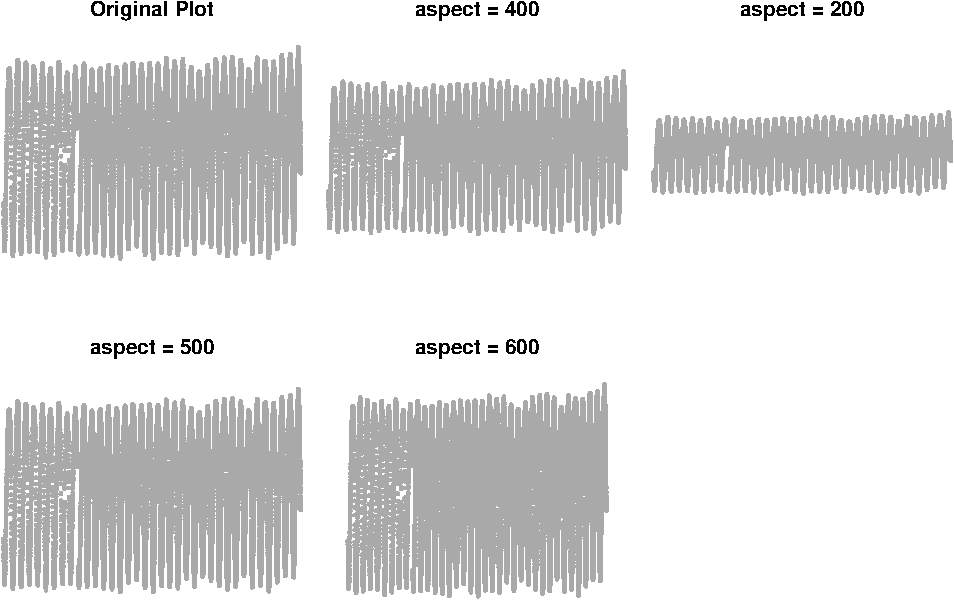
\includegraphics{a4_solutions_files/figure-latex/unnamed-chunk-24-1.pdf}

\begin{Shaded}
\begin{Highlighting}[]
\CommentTok{# Zooming with loon}
\KeywordTok{require}\NormalTok{(loon)}
\end{Highlighting}
\end{Shaded}

\begin{verbatim}
## Loading required package: loon
\end{verbatim}

\begin{verbatim}
## Loading required package: tcltk
\end{verbatim}

\begin{verbatim}
## 
## Attaching package: 'loon'
\end{verbatim}

\begin{verbatim}
## The following object is masked from 'package:graph':
## 
##     complement
\end{verbatim}

\begin{Shaded}
\begin{Highlighting}[]
\KeywordTok{l_plot}\NormalTok{(sea.ice, }\DataTypeTok{showScales=}\OtherTok{TRUE}\NormalTok{, }
     \DataTypeTok{size=}\FloatTok{0.3}\NormalTok{, }\DataTypeTok{glyph=}\StringTok{"ccircle"}\NormalTok{, }
     \DataTypeTok{color=}\StringTok{"darkgrey"}\NormalTok{)}
\end{Highlighting}
\end{Shaded}

\begin{verbatim}
## [1] ".l0.plot"
## attr(,"class")
## [1] "loon"
\end{verbatim}

The value of the extent of the Antartic sea ice stays within the same
range, but it continuously sharply decreasing and increasing over short
time periods.

\item 

Decomposition into a long term trend and a short term trend. First we
need to transform the data again.

\begin{Shaded}
\begin{Highlighting}[]
\NormalTok{sea.ice.xy <-}\StringTok{ }\KeywordTok{xy.coords}\NormalTok{(sea.ice)}
\NormalTok{y <-}\StringTok{ }\NormalTok{sea.ice.xy}\OperatorTok{$}\NormalTok{y}
\NormalTok{x <-}\StringTok{ }\NormalTok{sea.ice.xy}\OperatorTok{$}\NormalTok{x}
\CommentTok{# plotting x and y as before will yield the same plot, but}
\CommentTok{# with the dates lost.}
\CommentTok{#plot(x, y, cex=0.3, pch=19, col="darkgrey")}
\end{Highlighting}
\end{Shaded}

The data range from the beginning of 1979 to the end of 2014. The number
of years covered then is (2014-1979 + 1)=36. So each year is
approximately 1/36 of the series. A month is about 1/12 of this again.

\bitem    \item \textbf{(2 marks)} Using \texttt{loess(..)} as in class,
find a long term trend using \texttt{span=2/3}. Add this trend as a
curve in a different colour on top the points (as in the above plot).
Describe the fit.

\begin{Shaded}
\begin{Highlighting}[]
\NormalTok{ltfit =}\StringTok{ }\KeywordTok{loess}\NormalTok{(y}\OperatorTok{~}\NormalTok{x, }\DataTypeTok{span=}\DecValTok{2}\OperatorTok{/}\DecValTok{3}\NormalTok{)}
\NormalTok{ltpred =}\StringTok{ }\KeywordTok{predict}\NormalTok{(ltfit)}
\NormalTok{xord =}\StringTok{ }\KeywordTok{order}\NormalTok{(x)}
\KeywordTok{plot}\NormalTok{(x, y, }\DataTypeTok{col=}\StringTok{"grey70"}\NormalTok{, }\DataTypeTok{pch=}\DecValTok{19}\NormalTok{, }
     \DataTypeTok{main=}\StringTok{"Locating the Long Term Trend"}\NormalTok{)}
\KeywordTok{lines}\NormalTok{(x[xord], ltpred[xord], }\DataTypeTok{lwd=}\DecValTok{2}\NormalTok{, }\DataTypeTok{col=}\StringTok{"steelblue"}\NormalTok{)}
\end{Highlighting}
\end{Shaded}

\begin{center}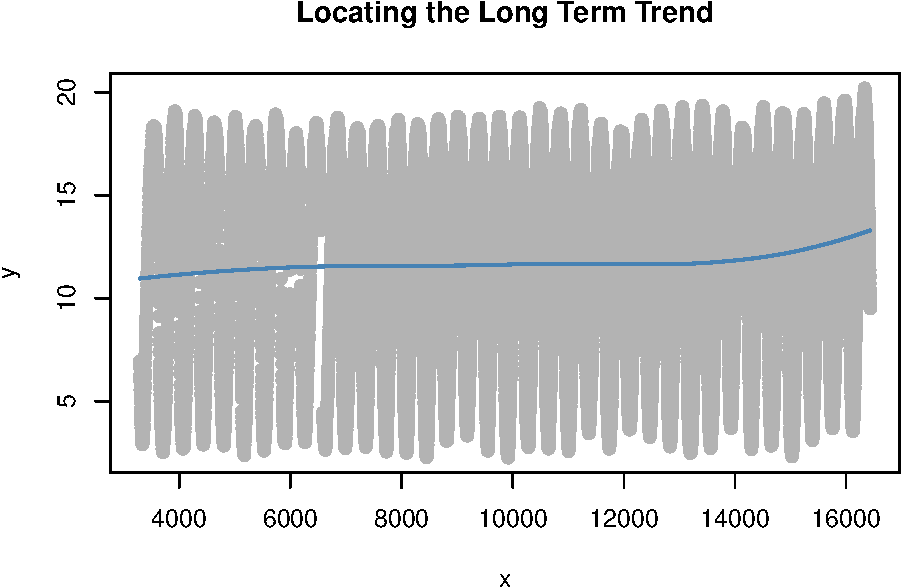
\includegraphics{a4_solutions_files/figure-latex/unnamed-chunk-27-1} \end{center}

The extent of Antarctic sea ice stays fairly consistent and stationary,
then there is a small jump upwards and the extent begins to trend
upwards (i.e.~increase) slowly.

\item 

\textbf{(2 marks)} Now fit a \texttt{loess} short term smooth with
\texttt{span=1/(36*12)} to the residuals from the long term trend. Plot
the residuals from the long-term trend and add the fitted short term
trend. Describe the fit.

\begin{Shaded}
\begin{Highlighting}[]
\NormalTok{resids =}\StringTok{ }\NormalTok{ltfit}\OperatorTok{$}\NormalTok{residuals}
\KeywordTok{plot}\NormalTok{(x, resids, }\DataTypeTok{col=}\StringTok{"grey70"}\NormalTok{, }\DataTypeTok{pch=}\DecValTok{19}\NormalTok{, }
     \DataTypeTok{main=}\StringTok{"Small Fit of Residuals from Long Term Trend"}\NormalTok{)}
\NormalTok{smfit =}\StringTok{ }\KeywordTok{loess}\NormalTok{(resids}\OperatorTok{~}\NormalTok{x, }\DataTypeTok{span=}\DecValTok{1}\OperatorTok{/}\NormalTok{(}\DecValTok{36}\OperatorTok{*}\DecValTok{12}\NormalTok{))}
\NormalTok{smpred =}\StringTok{ }\KeywordTok{predict}\NormalTok{(smfit)}
\KeywordTok{lines}\NormalTok{(x[xord], smpred[xord], }\DataTypeTok{lwd=}\DecValTok{2}\NormalTok{, }\DataTypeTok{col=}\StringTok{"steelblue"}\NormalTok{)}
\end{Highlighting}
\end{Shaded}

\begin{center}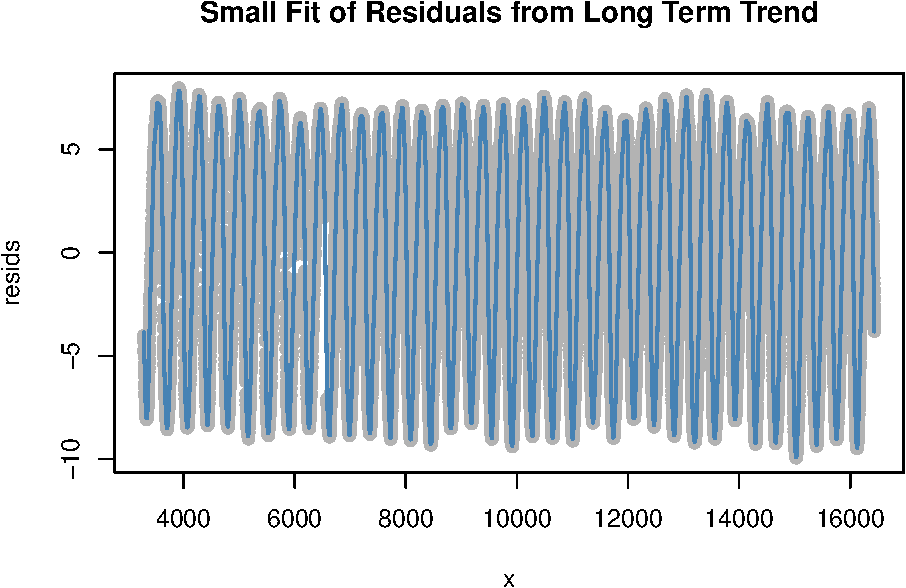
\includegraphics{a4_solutions_files/figure-latex/unnamed-chunk-28-1} \end{center}

The residuals exhibit a consistently seasonal trend - it trends upward
and the downwards very quickly for about every \(333\frac{1}{3}\) units
of x, staying with the range of about \([-10, 10]\).

\item 

\textbf{(3 marks)} Plot the residuals from the short-term trend.
Describe any patterns you find.

\begin{Shaded}
\begin{Highlighting}[]
\NormalTok{smresids =}\StringTok{ }\NormalTok{smfit}\OperatorTok{$}\NormalTok{residuals}
\KeywordTok{plot}\NormalTok{(x, smresids, }\DataTypeTok{col=}\StringTok{"grey70"}\NormalTok{, }\DataTypeTok{pch=}\DecValTok{19}\NormalTok{, }
     \DataTypeTok{main=}\StringTok{"Remaining residuals on x"}\NormalTok{)}
\NormalTok{rfit =}\StringTok{ }\KeywordTok{loess}\NormalTok{(smresids}\OperatorTok{~}\NormalTok{x, }\DataTypeTok{span=}\DecValTok{1}\OperatorTok{/}\NormalTok{(}\DecValTok{36}\OperatorTok{*}\DecValTok{12}\NormalTok{))}
\NormalTok{rpred =}\StringTok{ }\KeywordTok{predict}\NormalTok{(rfit)}
\KeywordTok{lines}\NormalTok{(x[xord], rpred[xord], }\DataTypeTok{lwd=}\DecValTok{2}\NormalTok{, }\DataTypeTok{col=}\StringTok{"steelblue"}\NormalTok{)}
\end{Highlighting}
\end{Shaded}

\begin{center}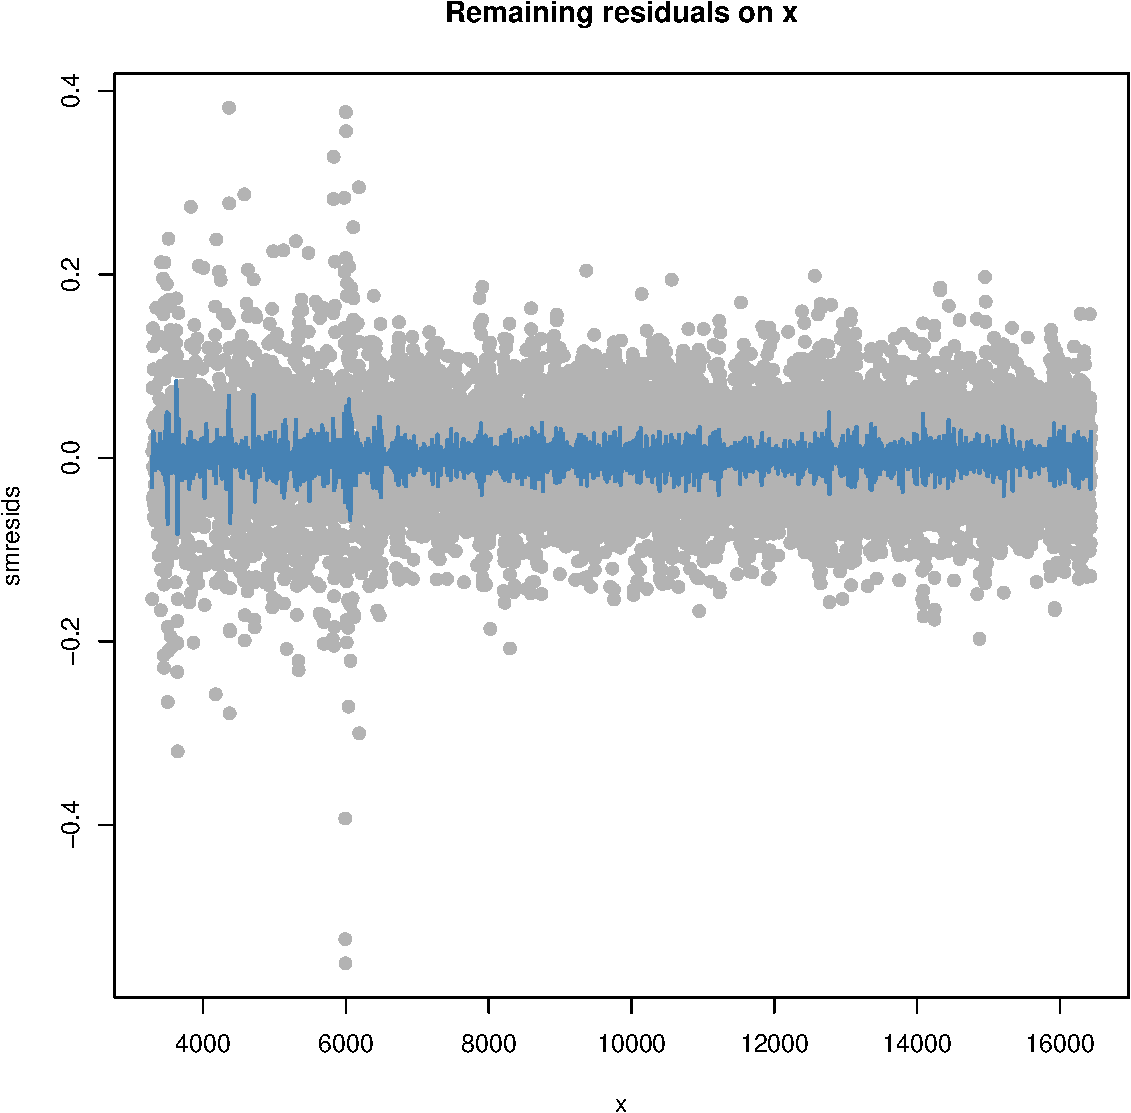
\includegraphics{a4_solutions_files/figure-latex/unnamed-chunk-29-1} \end{center}

There is no consistent trend in the plot - the remaining residuals are
too random to locate such a distinct pattern.

\item 

\textbf{(2 marks)} Explain your findings.

The graphs represent the different parts of the decomposition of the
time series model of the Antartic sea ice extent, with the first long
term trend of the extent being the main trend in the model, the short
term trend of the residuals representing the seasonality of the model,
and the remaining residuals representing the remaining randomness in the
model.

\eitem
\eenum

\item 

\textbf{Monthly averages} The original series was very irregular. Here
we replace it with a complete series using the average extent for each
month. This time series is created as follows.

\begin{Shaded}
\begin{Highlighting}[]
\NormalTok{months <-}\StringTok{ }\KeywordTok{unique}\NormalTok{(seaice}\OperatorTok{$}\NormalTok{Month)}
\NormalTok{nmonths <-}\StringTok{ }\KeywordTok{length}\NormalTok{(months)}
\NormalTok{years <-}\StringTok{ }\KeywordTok{unique}\NormalTok{(seaice}\OperatorTok{$}\NormalTok{Year)}
\NormalTok{nyears <-}\StringTok{ }\KeywordTok{length}\NormalTok{(years)}
\CommentTok{# check the beginning and the end months.}
\NormalTok{seaice[}\DecValTok{1}\NormalTok{,]}
\end{Highlighting}
\end{Shaded}

\begin{verbatim}
##   Year Month Day Extent
## 1 1979     1   2  6.945
\end{verbatim}

\begin{Shaded}
\begin{Highlighting}[]
\NormalTok{seaice[}\KeywordTok{nrow}\NormalTok{(seaice),]}
\end{Highlighting}
\end{Shaded}

\begin{verbatim}
##       Year Month Day Extent
## 11552 2014    12  31  9.508
\end{verbatim}

\begin{Shaded}
\begin{Highlighting}[]
\NormalTok{maxN <-}\StringTok{ }\NormalTok{nmonths }\OperatorTok{*}\StringTok{ }\NormalTok{nyears}
\CommentTok{# place holder}
\NormalTok{iceMonthly <-}\StringTok{ }\KeywordTok{vector}\NormalTok{(}\StringTok{"numeric"}\NormalTok{, }\DataTypeTok{length=}\NormalTok{maxN)}
\ControlFlowTok{for}\NormalTok{ (i  }\ControlFlowTok{in} \DecValTok{1}\OperatorTok{:}\NormalTok{nyears) \{}
\NormalTok{  year <-}\StringTok{ }\NormalTok{seaice[,}\StringTok{"Year"}\NormalTok{] }\OperatorTok{==}\StringTok{ }\NormalTok{years[i]}
\NormalTok{  iceyear <-}\StringTok{ }\NormalTok{seaice[year,}\KeywordTok{c}\NormalTok{(}\StringTok{"Month"}\NormalTok{,}\StringTok{"Extent"}\NormalTok{)]}
  \ControlFlowTok{for}\NormalTok{ (j }\ControlFlowTok{in} \DecValTok{1}\OperatorTok{:}\NormalTok{nmonths) \{}
\NormalTok{    index <-}\StringTok{ }\NormalTok{(i}\OperatorTok{-}\DecValTok{1}\NormalTok{) }\OperatorTok{*}\StringTok{ }\NormalTok{nmonths }\OperatorTok{+}\StringTok{ }\NormalTok{j}
\NormalTok{    selection <-}\StringTok{  }\NormalTok{iceyear[,}\StringTok{"Month"}\NormalTok{] }\OperatorTok{==}\StringTok{ }\NormalTok{months[j]}
\NormalTok{    iceMonthly[index] <-}\StringTok{ }\KeywordTok{mean}\NormalTok{(iceyear[selection,}\StringTok{"Extent"}\NormalTok{])}
\NormalTok{  \}}
\NormalTok{\}}
\CommentTok{#  Now we create a time series object}
\NormalTok{ice <-}\StringTok{ }\KeywordTok{ts}\NormalTok{(iceMonthly, }\DataTypeTok{start=}\KeywordTok{c}\NormalTok{(}\DecValTok{1979}\NormalTok{,}\DecValTok{1}\NormalTok{), }\DataTypeTok{frequency=}\DecValTok{12}\NormalTok{)}
\end{Highlighting}
\end{Shaded}

Conduct a seasonal trend analysis on \texttt{ice} using the built-in
\texttt{stl(...)} function with parameters \texttt{s.window=11},
\texttt{s.degree=1}, and \texttt{t.degree=1}.

\benum
\item \textbf{(3 marks)} Plot the output of \texttt{stl} and describe
your findings.

\begin{Shaded}
\begin{Highlighting}[]
\KeywordTok{plot}\NormalTok{(}\KeywordTok{stl}\NormalTok{(ice, }\DataTypeTok{s.window=}\DecValTok{11}\NormalTok{,}
         \DataTypeTok{s.degree=}\DecValTok{1}\NormalTok{, }\DataTypeTok{t.degree=}\DecValTok{1}\NormalTok{))}
\end{Highlighting}
\end{Shaded}

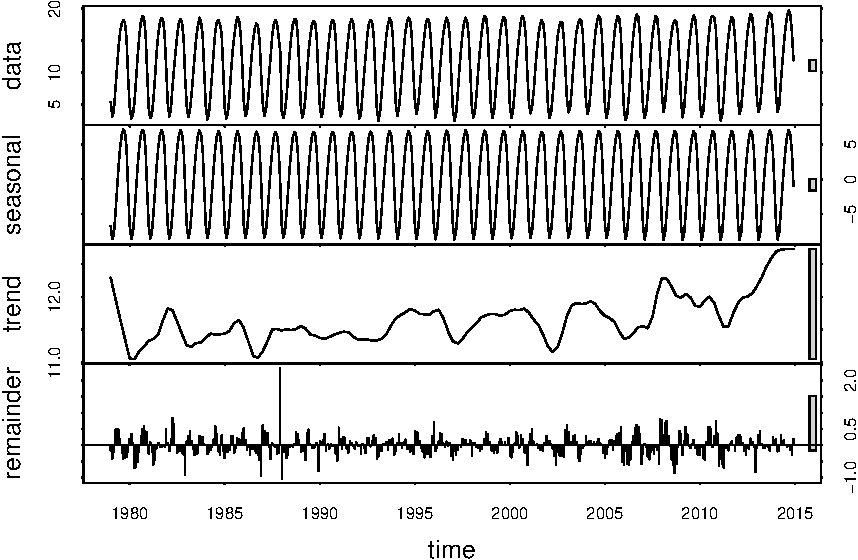
\includegraphics{a4_solutions_files/figure-latex/unnamed-chunk-31-1.pdf}

The long term trend of the data is cyclical - the short-term
trends/cycles where the extent decreases and the increases again don't
repeat regularly.

\item 

\textbf{(2 marks)} Compare the output above with the decomposition of
the irregular time series in part (a).

The shape of the seasonal portion of the diagram and randomness of the
remainder is consistent with what was plotted in part (a) for the short
term smooth of residuals and the plot of the remaining residuals
respectively.

However, the main trend of the two questions are different, with the
trend in part (a) having exhibited a stationary trend and the trend in
part (b) being more cyclical. This is due to the irregularity of the
data used in part (a), with part (b) showing the true trend of the data
as the ice extents for the missing dates in part (a) have been accounted
for.

\eenum
\eenum

\eenum


\end{document}
